% !TeX encoding = UTF-8
% !TeX spellcheck = en_GB

%%% Add [final] option to the report class to switch between draft and final version of the report
%%% Use [narrowmargin] to enable narrow margins - this may impair readability.
%\documentclass[a4paper,12pt,draft]{include/intocpsreport}   %Or
\documentclass[a4paper,12pt,final]{include/intocpsassociation}   %Or
% intocpslargereport if chapters are required.
%
%
%
\usepackage[T1]{fontenc}
\usepackage[utf8]{inputenc}
\usepackage{longtable}
%\usepackage{tikz-uml}
\usepackage{framed}
\usepackage{subcaption}
\usepackage[hyphenbreaks]{breakurl}
\usepackage{color}
\usepackage{amsmath}
\usepackage{courier}
\usepackage{xspace}
\usepackage{cleveref}
\usepackage{subcaption}
\usepackage{textcomp} % Used for 20-sim section \textrightarrow
%\usepackage{showframe}

\usepackage{listings}
%%% listings-modelica.cfg
%% Copyright 2014 Martin Sjoelund, Dietmar Winkler
%
% This work may be distributed and/or modified under the
% conditions of the LaTeX Project Public License, either version 1.3
% of this license or (at your option) any later version.
% The latest version of this license is in
%   http://www.latex-project.org/lppl.txt
% and version 1.3 or later is part of all distributions of LaTeX
% version 2005/12/01 or later.
%
% This work has the LPPL maintenance status `maintained'.
%
% The Current Maintainer of this work is Dietmar Winkler
%
% Code repository https://github.com/modelica-tools/listings-modelica
%
% This work consists of the file listings-modelica.cfg

\lstdefinelanguage{modelica}
{
  morekeywords=[1]{
    algorithm,and,annotation,as,assert,block,break,case,class,connect,connector,
    constant,constrainedby,der,discrete,each,else,elseif,elsewhen,encapsulated,
    end,enumeration,equality,equation,expandable,extends,external,failure,final,
    flow,for,function,guard,if,import,in,initial,inner,input,List,local,loop,
    match,matchcontinue,model,not,operator,Option,or,outer,output,package,parameter,
    partial,protected,public,record,redeclare,replaceable,return,stream,
    subtypeof,then,Tuple,type,uniontype,when,while},
  morekeywords=[2]{true, false},
  % Do not make true,false keywords because fn(true,x, false ) shows up as fn(true,x, *false*)
  sensitive=true,
  comment=[l]//,
  morecomment=[s]{/*}{*/},
  alsodigit={.,-},
  morestring=[b]',
  morestring=[b]",
}[keywords,comments,strings]

\definecolor{keywordcolor1}{rgb}{0,0,.4}
\definecolor{keywordcolor2}{rgb}{.90,0,0}
\definecolor{stringcolor}{rgb}{0.133,0.545,0.133}
% \definecolor{listingbgcolor}{rgb}{0.95,0.95,0.95}

\lstset{
	frame=trBL,
  breaklines=true,
  language=modelica,
  basicstyle=\ttfamily,
  keywordstyle=[1]\color{keywordcolor1}\bfseries,
  keywordstyle=[2]\color{keywordcolor2},
  stringstyle=\color{stringcolor},
%  backgroundcolor=\color{listingbgcolor},
  framexleftmargin=5mm,
  frameround=fttt,
  xleftmargin=5mm,
  xrightmargin=5mm,
  showstringspaces=false,
}

\lstset{breaklines=true,label=}
% \lstset{basicstyle=\ttfamily}

\newcommand{\code}[1]{\texttt{\hyphenchar%
\font45%
\sloppy%
\fontdimen2\font=0.4em%
\fontdimen3\font=0.2em%
\fontdimen4\font=0.1em%
\fontdimen7\font=0.1em%
 #1}}
 
 


\usepackage{acronym}
\acrodef{mdt}[MDT]{MAN Diesel \& Turbo}
\acrodef{sil}[SIL]{Software In the Loop}
\acrodef{ct}[CT]{Continuous-Time}
\acrodef{mdse}[DSE]{Dynamic Simulation Environment}
\acrodef{hil}[HIL]{Hardware In the Loop}
\acrodef{intocps}[INTO-CPS]{Integrated Tool Chain for Model-based Design of Cyber-Physical Systems}
\acrodef{os}[OS]{Operating System}
\acrodef{fmi}[FMI]{Functional Mock-up Interface}
\acrodef{coe}[COE]{Co-simulation Orchestration Engine}  
\acrodef{egr}[EGR]{Exhaust Gas Recirculation}



% The VDMlisting package loads the times package which changes the font so we just mark it as loaded to prevent the load.
\makeatletter
\@namedef{ver@times.sty}{}% a fake for a "loaded" package
\makeatother
\usepackage{vdmlisting}

%% Define listing environment for XML
\definecolor{gray}{rgb}{0.4,0.4,0.4}
\definecolor{darkblue}{rgb}{0.0,0.0,0.6}
\definecolor{cyan}{rgb}{0.0,0.6,0.6}

\lstset{
  basicstyle=\footnotesize\ttfamily,
  columns=fullflexible,
  showstringspaces=false,
  commentstyle=\color{gray}\upshape
}

\lstdefinelanguage{XML}
{
  morestring=[b]",
  morestring=[s]{>}{<},
  morecomment=[s]{<?}{?>},
  stringstyle=\color{black},
  identifierstyle=\color{darkblue},
  keywordstyle=\color{cyan},
  morekeywords={xmlns,version,type}% list your attributes here
}


\lstnewenvironment{xml}[1][]{\lstset{  language=XML,
  morekeywords={encoding, xs:schema,xs:element,xs:complexType,xs:sequence,xs:attribute}}\lstset{#1}}
{}

%% end listing environment for XML
%
%
%
\def\draftnote#1{\noindent\smallskip\framebox{\begin{minipage}{0.95\columnwidth}\color{red}#1\end{minipage}}\smallskip\par}
\newenvironment{draftnoteenv}{\noindent\smallskip\begin{framed}\begin{minipage}{0.95\columnwidth}\color{red}}{\end{minipage}\end{framed}\smallskip\par}
\newenvironment{assumption}{\noindent\smallskip\color{blue}\begin{framed}\begin{minipage}{0.95\columnwidth}}{\end{minipage}\end{framed}\smallskip\par}
%
%
%
\newcommand{\revisit}[1]{\textcolor{red}{\pmb{[[[}\@ #1\@ \pmb{]]]}}}
\newcommand{\intoapp}{INTO-CPS Application}
\newcommand{\into}{INTO-CPS\xspace}


% Enable/Disable comments.
\newif\ifcomments
\commentstrue

\newcommand{\claudio}[1]{%
\ifcomments %
{\bfseries \scriptsize \color{red} Claudio: #1} %
\else %
 %
\fi%
}%

%
%
%\reportnumber{D4.3a}
\reporttitle{The INtegrated TOolchain for Cyber-Physical Systems (INTO-CPS): a Guide}
%\reporttitle{The INTO-CPS Manifesto}
%\reporttitle{User Manual for the INTO-CPS Tool Chain}
%\shortreporttitle{The INTO-CPS Manifesto}  %To use if report title is too long for header
\shortreporttitle{The INTO-CPS Guide}  %To use if report title is too long for header%
%
%
%%% Set document release class as appropriate
%%% e.g. Public, Restricted, Programme Participant
\reportstatus{Public}
%
%
%
%%% If document is a deliverable, this flag should be commented out
%%% e.g. %\technotetrue
%%% If report is a technical report, leave uncommented
%%% e.g. \technotetrue
%\technotetrue % Comment out as appropriate
%
%
\def\into{INTO-CPS}
\def\SG{Smart Grid}
\def\term#1{\textbf{\emph{#1}}}
%
%
%
%
\submissiondate{October, 2018}
\contributors{
Peter Gorm Larsen, Aarhus University\\
John Fitzgerald, Newcastle University\\
Jim Woodcock, University of York\\
Christian K\"{o}nig, TWT\\
Stylianos Basagiannis, UTRC\\
Etienne Brosse, Softeam\\
Cláudio Gomes, University of Antwerp\\
Jos\'{e} Cabral, Fortiss \\
Hugo Daniel Macedo, Aarhus University\\
Casper Thule, Aarhus University\\
Andrey Sadovykh, Softeam\\
Constantin-Bala Zamfirescu,``Lucian Blaga'', University of Sibiu\\
Mihai Neghina, ``Lucian Blaga'', University of Sibiu\\
Ken Pierce, Newcastle University\\
Carl Gamble, Newcastle University\\
Richard Payne, Newcastle University
}
%
%
%
\editors{
  Peter Gorm Larsen, Aarhus University\\
  John Fitzgerald, Newcastle University
}
%
%
%
%\reviewers{Ken Pierce, UNEW\\
%Kangfeng Ye, UY\\
%Luis Diogo Couto, UTRC}
%
%
%
%% Version details
% #1: version
% #2: date
% #3: author
% #4: description
\addversion{0.01}{23-04-2018}{Peter Gorm Larsen}{Initial version.}

%
%
\begin{document}
\maketitle
%
%
%
%%%% Document abstract page %%%%
\section*{Abstract}
\label{sec:abstract}
%
%\fbox{John Fitzgerald}
The successful design, implementation and maintenance of cyber-physical systems requires collaboration between diverse engineering disciplines and organisations, each of which may use radically different tools and notations.
The INtegrated TOolchain for Cyber-Physical Systems (INTO-CPS) is an open framework that permits the coupling of tools for model-based CPS engineering. Its formal foundations and the use of the Functional Mockup Interface standard permit the coherent integration of tools that describe CPS architecture, data, and discrete-event and continuous-time models of system elements. This allows engineers to produce collaborative models (co-models) and undertake co-simulation of behaviour at the whole-CPS level. It permits the machine-assisted trade space analysis, analytic detection and resolution of defects, generation of tests and of code. The value of the approach in reducing time to market and particular in reducing the number of physical prototype iterations required in product development, has been demonstrated in industry.

This report is a guide to INTO-CPS. It includes a review of the challenges facing CPS engineers today and argues for open and integrated toolchains. The INTO-CPS technology is described briefly, and the semantic foundation of the approach are \claudio{``is'', instead of ``are''?} outlined. Methods for exploiting the toolchain within existing systems engineering processes are outlined, and the current toolchain itself is described alongside several real \claudio{I would remove ``real'' from here. It seems we're trying too hard to show that they are real\ldots} industry studies. We argue that the future of CPS engineering relies on the integration of existing tools and processes, and we offer a potential roadmap for future research in the field, notably in realising the potential of co-models as learning digital twins \claudio{It's not clear what ``learning digital twins'' here means\ldots is it AI enhance digital twins?}.
\newpage
%
%%%% Document table of contents page %%%%
\tableofcontents
\newpage
%
%
%
%%%% Document Content %%%%
%% \chapter{Chapter Title} %% if intocpslargereport is in use
%\begin{assumption}
%
%
%
%!TEX root = ../INTO-CPS-Manifesto.tex

\section{Introduction}\label{sec:intro}

%\fbox{Peter Gorm Larsen}

Cyber-Physical Systems (CPSs) present major business and societal
opportunities in a variety of application areas--- \emph{if} they can be developed economically~\cite{Cengarle&13}. Model-Based Development (MBD) has the potential to enhance the development of CPSs, increasing the competitiveness of industry by shortening time to market and reducing development costs. In the interface between disciplines, different formalisms and technical cultures meet, and the traditional approaches for designing systems vary significantly among the relevant fields. Some researchers advocate for describing such hybrid systems using a single formalism/tool \cite{Ptolemaeus14,Platzer18}, but here we believe that it is better to enable stakeholders with different disciplinary backgrounds to produce their constituent models using their preferred formalism/tool and then enable joint analysis using co-simulation \cite{Gomes&18} and ensuring that there is an underlying common foundation for all of them.
Even the proposals for a single \cite{Ptolemaeus14,Platzer18} recognise that one cannot expect different stakeholders to learn the same formalism. Instead, they propose a formalism that integrates multiple sub-formalisms, to ensure that the result can cover a wide range of paradigms.

Different stakeholders can produce constituent models of the parts they are responsible for. The combination of the different constituent models forms the CPS model.
The main challenge is to ensure that such constituent models connect and thus can be combined in different analysis conducted of the behaviour of the CPS in its desired surroundings, typically called its environment.
%\claudio{The prev sentence is also trying to do too much!}
Since the design of the CPSs depends on the ability to connect the behaviours of its constituent models, the main challenge is to make sure these results are trustworthy.
%Different formalisms are usually
%supported by different tools running on different Operating Systems (OSs).

Different research projects have targeted the development of chains of tools which collectively would enable the envisaged combination of different formalisms and tools in the development of CPSs. The DESTECS\footnote{This is an acronym for ``Design Support and Tooling for Embedded Control Software'', see \url{http://destecs.org/}.} project \cite{Broenink&10} combined the Overture/VDM tool \cite{Larsen&10a} with the 20-sim tool \cite{Kleijn06} with a dedicated co-simulation combination with a Crescendo tool \cite{Fitzgerald&14c}. The MODELISAR project\footnote{See \url{https://itea3.org/project/modelisar.html}.} developed an open standard for interfacing between different constituent models called the Functional Mockup Interface (FMI) enabling co-simulation between any tool supporting this standard maintained by the Modelica Association\footnote{See \url{https://www.modelica.org/}.}. The INTO-CPS project\footnote{See \url{http://projects.au.dk/into-cps/}.} took this further with a tool chain going all the way from requirements to final realisations using the FMI standard. This developed the INTO-CPS technology which consists of 1) a common semantic foundation, 2) a methodology with guidelines for the development of CPS and 3) an open tool chain.
\claudio{Maybe you can summarize the above in a table. Maybe as in Table~\ref{tab:projects}.}

\begin{table}[htb]
  \scriptsize
  \caption{Summary of research activities in the field of co-simulation in recent years. \claudio{Taken from a journal paper which has been submitted but not accepted yet. Maybe need to cite it like that\ldots}}
  \label{tab:projects}
  \begin{tabular}{llp{0.55\textwidth}}
  \textbf{Project} & \textbf{Duration} & \textbf{Goals} \\ \hline
  COSIBA~\cite{cosibas} & 2000--2002 &  Formulate a co-simulation backplane for coupling electronic design automation tools,  supporting different abstraction levels. \\
  ODETTE~\cite{odette} & 2000--20003 &  Develop a complete co-design solution including hardware/software co-simulation and synthesis tools. \\
  MODELISAR~\cite{modelisar} & 2008--2011 &  Improve the design of embedded software in vehicles. \\
  DESTECS~\cite{destecs} & 2010--2012 &  Improve the development of fault-tolerant embedded systems. \\
  INTO-CPS~\cite{intocps} & 2015--2017 &  Create an integrated tool chain for Model-Based Design of CPS with FMI.  \\
  ACOSAR~\cite{acosar} & 2015--2018 &  Develop a non-proprietary advanced co-simulation interface for real time system integration.  \\
  OpenCPS~\cite{opencps} & 2015--2018 &  Improve the interoperability between Modelica, UML and FMI.  \\
  ERIGrid~\cite{erigrid} & 2015--2020 &  Propose solutions for Cyber-Physical Energy Systems through co-simulation.  \\
  PEGASUS~\cite{pegasus} & 2016--2019 &  Establish standards for autonomous driving. \\
  CyDER~\cite{cyder} & 2017--2020 &  Develop a co-simulation platform for integration and analysis of high PV penetration. \\
  EMPHYSIS~\cite{emphysis} & 2017--2020 &  Develop a new standard (eFMI) for modeling and simulation environments of embedded systems.  \\ 
  \hline
  \end{tabular}%
\end{table}


Before the end of the INTO-CPS project, the Intellectual Property (IP) developed was transferred to the non-profit INTO-CPS Association\footnote{This is registered as a legal entity in Denmark, see \url{into-cps.org/}.}. The Association maintains and further develops the INTO-CPS technology, and grows the open tool chain by adding additional tools from its partners, while keeping the documentation and tutorial material up to date. 
%It attempts to ensure that the different tools are kept in sync and that the importable examples expressed using diverse notations and tools are kept up to date.
%\claudio{This last sentence seems redundant.}

Since this guide is meant as a general introduction to INTO-CPS it is written such that it should be relatively easy to jump around and read different sections of interest. This guide to INTO-CPS begins with an overview of challenges in the engineering of CPSs in Section~\ref{sec:challenges}. Then Section~\ref{sec:nutshell} provides a short overview of the INTO-CPS project in a nutshell. Section~\ref{sec:foundations} gives an overview of the CPS foundations; Section~\ref{sec:method} gives an overview of the CPS methodology; and Section~\ref{sec:toolchain} an overview of the tool chain. The industrial use of the INTO-CPS technology is summarised in Section~\ref{sec:casestudies}. Finally, Section~\ref{sec:related} provides an overview of related work, and Section~\ref{sec:future} looks at potential future directions for the INTO-CPS technology. 
There are two appendices: Appendix~\ref{appendix:acronyms} provides a list of acronyms,  
%Appendix~\ref{appendix:principles} provides a common definition of the main terms used in the INTO-CPS documentation 
and Appendix~\ref{appendix:tools} is an overview of the individual tools used in the INTO-CPS tool chain.
%There are three appendices: Appendix~\ref{appendix:acronyms} provides a list of acronyms; Appendix~\ref{appendix:principles} provides a common definition of the main terms used in the INTO-CPS documentation and Appendix~\ref{appendix:tools} is an overview of the individual tools used in the INTO-CPS tool chain.

%Systems composed of closely coupled computing and physical elements are becoming increasingly important in the modern world. For society and citizens, the potential of such smart systems to deliver more efficient, sustainable and resilient services is enormous.  Such Cyber-Physical Systems (CPSs) are characterised by a complex architecture and a design process involving several diverse science and engineering disciplines. In the interface between disciplines, different formalisms and technical cultures meet, and the traditional approaches for designing systems vary significantly among the relevant fields.
%\claudio{It's not clear how the previous sentence relates to the next. Is it the cause of the vast design space? It seems to be more related to the two last sentences of this paragraph.}
%The developer of a CPS faces a large design space that is hard to cover with hardware prototypes \claudio{maybe add: and physical experiments} due to the high cost of their implementation. Common workflows to assist the engineering of CPSs with a model-based approach, and the necessary tools, are currently lacking. Different stakeholders can produce models of the parts they are responsible for, and we will call these constituent models that together form the entire CPS.
%
%\claudio{This paragraph seems to be the continuous of the previous one (but the previous one has a gap, and should maybe be splitted).
%Anyhow, the logical workflow is a bit confusing. Maybe we should go bottom up: first explain the there are diverse disciplines, and that each has its methods, formalisms, and jargon, and then explain that these need to interact and collaborate, in order to successfully develop a CPS. This then leads us to the need for into-cps.}
%The design of CPSs involves the usage of results obtained
%using a combination of different formalisms serving different engineering
%disciplines. Different formalisms are usually
%supported by different tools running on different Operating Systems (OSs).
%
%In this manifesto we put forward the idea of combining different formalisms and
%respective supporting tools by means of a tool chain. A tool chain allows the
%practitioner to easily combine the results from the various fields during the
%design process.  Our view is that it is best to enable different disciplinary experts to use the tools they are most familiar with and
%integrating the different constituent models by building an environment automating the tool chain
%interaction, accessibility, and unifying the entry point to it.
%\claudio{If the motivation is clearly provided in the previous paragraphs, then this last sentence should be redundant.}
%
%In such unified environment of several tools, users keep their usual patterns
%of interaction with their familiar tool(s) available in the tool chain.
%\claudio{The next sentence says the same thing as the previous one.}
%Instead of having to learn a new formalism, the different disciplinary experts can stay with the tools they are most familiar with and they find most natural to create the constituent models requires for their work.
%The chain of tools then needs also to enable each individual of seeing the consequences of changes locally in a global context where the other constituent models are incorporated.
%\claudio{I think this paragraph should not need to exist, if the problem is well motivated. These are all pressing needs in the current development of CPS.
%So the logical flow should be ``MOTIVATION (pressing needs) -> Solution (it should be clear why this is a solution, we don't need to justify more)''.}
%
%Naturally, such different constituent models needs to interface to each other and here we make use of a de-facto standard originating in the automotive industry called the Functional-Mockup Interface (FMI).
%\claudio{The next sentence says the same thing as the previous one.}
%Thus, the different tools in the INTO-CPS tool chain are able to interact with other tools directly or indirectly using the FMI standard.
%\claudio{The next couple of sentences seems to be an afterthought. Maybe they should be put in a different paragraph, and the problem that the traceability solves should be described in the motivation section.}
%In order also to be able to trace artefacts from different constituent models and results generated from analysis using different tools another standard called the Open Services for Lifecycle Collaboration (OSLC) is used. This enables seeing and documenting the dependencies between different versions of different constituent models and local or global analysis conducted about them.
%
%\claudio{What's the point of the next sentence?}
%It is hard for a single person to master all the components of the tool chain, but fortunately that is not required.
%The mastering of tool chains involves the management of the whole set
%of models and inputs/results for each of the tools. In addition, the conversion
%of results, traceability of changes and keeping track of the user interactions
%need also to be taken into account.
%\claudio{The next sentence is one of the motivations for the INTO-CPS association\ldots It should be in a paragraph by itself.}
%Moreover, given the evolving nature of
%each of the tools, the task of managing the tool chain while ensuring the
%dependencies of each of the tools and their interoperability becomes too
%complex. The INTO-CPS Association attempts to ensure that the different tools are kept in sync and that the importable examples expressed in a collection of notations using different tools \claudio{Do we need to say ``expressed in a collection of notations using different tools''? That seems redundant.} (these are called multi-models \claudio{We don't need to define a new term here, if we are not going to use it in this section.}) are kept up to date.
%
%%Practice shows users are more receptive to a  push-button approach when it is
%%time to combine their results with the other tools.
%
%\claudio{Why did we switch from talking about the into-cps association, to the into-cps tool?
%Why not start with the tecnology, and end with the into-cps association? Because we start with the tecnological problems\ldots}
%The INTO-CPS technology builds upon a frontend application which was developed following the
%unified entry point idea.  The INTO-CPS application allows the user to fetch
%the different tools, checkout multi-models from repositories, orchestrate the
%several tools run, and organise the results/interactions.  This reduces the
%challenges of mastering the complexity essentially to a push-button effort when the multi-models have been produced by different disciplinary experts.
%



\clearpage
\section{Challenges in Engineering CPSs}\label{sec:challenges}

%\fbox{John Fitzgerald - rough notes at this point}

The vision underpinning \into\ is that teams of developers from diverse disciplines and organisations are enabled to work together to converge more rapidly than today on system designs that perform optimally. Realising this vision requires methods and tools that each discipline and organisation to make its contribution without compromising its intellectual property or significantly altering its well-tried and established techniques. It should be possible to federate these diverse design artefacts to allow analysis of the system-level consequences of design decisions made in any one domain, and the trade-offs between them. How, then, can we support such multidisciplinary design with semantically well-founded approaches in a cost-effective manner? In general we believe that there are a number of areas where there are challenges in the proper engineering of CPSs. These are described below in separate subsections.

\subsection{The challenge of time to market}

There is a clear need for model-based methods to permit early design space exploration, optimisation and experimentation without delaying the time from initial idea towards the launch of a new product to the market. We feel that the main areas of relevance here are:

\begin{description}
\item[Faster route to market for engineering CPSs:] In a highly active CPS marketplace, getting the right solution first time is essential. We believe that the interoperability of tools in the INTO-CPS tool suite enables a more agile close collaboration between stakeholders with diverse disciplinary backgrounds.
\item[Exploring large design spaces efficiently:] CPS design involves making design decisions in both the cyber and physical domains. Trade-off analysis can be challenging. Co-simulation enables the systematic exploration of large design spaces in the search for optimal solutions.
\item[Limiting expensive physical tests:] CPS development often relies on the expensive production and evaluation of a series of physical prototypes. Co-simulation enables users to focus on testing different models of CPS elements in a virtual setting, gaining early assessment of CPS-level consequences of design decisions.
\end{description}

\subsection{The challenge of diversity}

In the INTO-CPS project we start from the view that disciplines such as software, mechatronic and control engineering have evolved notations and theories that are tailored to their needs, and that it is undesirable to suppress this diversity by enforcing uniform general-purpose models~\cite{Fitzgerald&15,Larsen&16e}. The goal, then, must be to allow the effective federation of highly diverse design models.

\subsection{The challenge of collaboration}

There is a clear need to provide mechanisms to support collaborative model-base engineering without compromising the independence of contributors. We feel that the main areas of relevance here are:

\begin{description}
\item[Avoiding vendor lock-in by open tool chain:] Some commercial solutions provide at least a part of the functionality provided by the INTO-CPS tool chain with a high level of interoperability. However, in particular for Small and Medium-sized Enterprises (SMEs), there is a risk of being restricted in the choice of specialist tools.
\item[Traceability and Provenance:] CPS development often relies on the expensive production and evaluation of a series of physical prototypes. Co-simulation enables users to focus on testing different models of CPS elements in a virtual setting, gaining early assessment of CPS-level consequences of design decisions.
\end{description}



To the CPS engineer, the system of interest includes both computational and physical elements, so the foundations, methods and tools of CPS engineering should incorporate both the Discrete-Event (DE) models of computational processes, and the continuous-value and Continuous-Time (CT) formalisms of physical dynamics engineering. Our approach is to support the development of collaborative models (\emph{co-models}) containing DE and CT elements expressed in diverse notations, and to support their analysis by means of co-simulation based on a reconciled operational semantics of the individual notations' simulators \cite{Fitzgerald&14c}. This enables exploration of the design space and allows relatively straightforward adoption in businesses already exposed to some of these tools and techniques. The idea is to enable co-simulation of extensible groups of semantically diverse models, and at the same time the semantic foundations are extended using Unifying Theories of Programming (UTP) to permit analysis using advanced meta-level tools that are primarily targeted towards academics and thus not considered as a part of the industrial INTO-CPS tool chain.


\clearpage
\section{INTO-CPS in a Nutshell}\label{sec:nutshell}

%\fbox{Peter Gorm Larsen}


To address the challenges presented above in Section~\ref{sec:challenges}, INTO-CPS project has created an integrated ``tool chain'' for comprehensive model-based design of CPSs. The tool chain supports multidisciplinary, collaborative modelling of CPSs from requirements, through simulation of multiple heterogeneous models that represent the physical elements as well as the computational parts of the system, down to realisation in hardware and software, enabling traceability at all stages of the development as outlined in figure~\ref{fig:intooverview}.

\begin{figure}[ht]
\centering
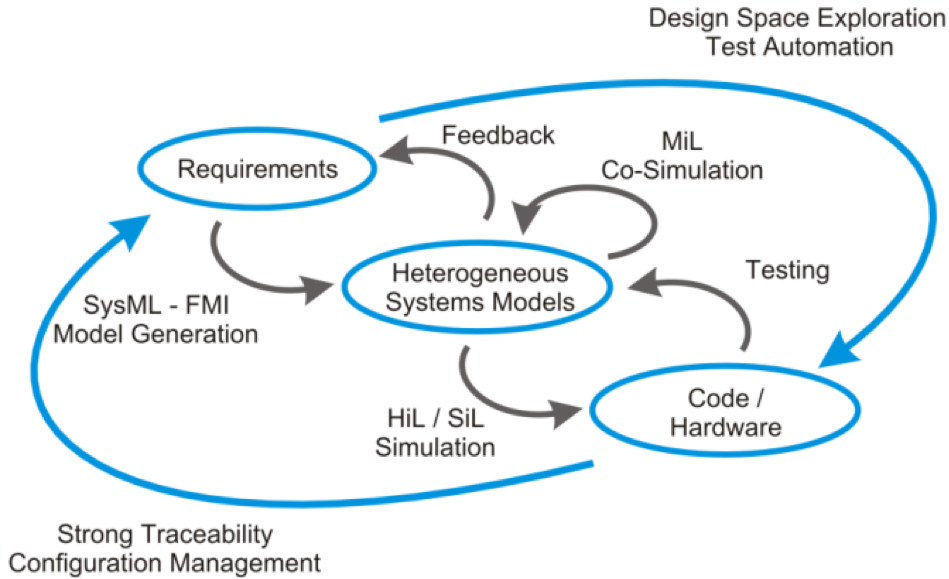
\includegraphics[width=\textwidth]{./figures/INTOoverview}
\caption{Connections in the INTO-CPS tool chain.}
\label{fig:intooverview}
\end{figure}

The goals of the INTO-CPS project have been to:
\begin{enumerate}
\item Build an open, well-founded tool chain for multidisciplinary model-based design of CPS that covers the full development life cycle of CPS.
\item Provide a sound semantic basis for the tool chain.
\item Provide practical methods in the form of guidelines and patterns that support the tool chain.
\item Demonstrate the effectiveness of the methods and tools in an industrial setting in a variety of application domains.
\item Form an INTO-CPS Association to ensure that results extend beyond the life of the project.
\end{enumerate}

\subsection{How INTO-CPS works}

The INTO-CPS project had a consortium consisting of 11 partners (four universities, seven companies) who contribute with complementary knowledge, baseline technologies and applications. The baseline technologies support systems modelling (Modelio), modelling and simulation of physical systems (OpenModelica, 20-sim), discrete-event modelling and simulation (Overture), Co-Simulation (Crescendo, TWT Co-Simulation engine) and test automation (RT-Tester). These baseline technologies enable both descriptions of Discrete Event (DE) models as well as Continuous-Time (CT) models. Any number of such constituent models may be combined in a hybrid setting using the INTO-CPS technology. Advancing over technologies commonly used today in industry, INTO-CPS provides an open tool chain that enables the following:

\begin{enumerate}
\item Providing a faster route to market for CPS products where control aspects depend upon the development of physical elements (e.g.\ mechanical parts) that typically take a long time to be developed.
\item Avoiding vendor lock-in by having an open tool chain that can be extended and used in different ways. Although it is well-founded it is based on pragmatic principles where a trade-off between accuracy and speed of analysis is enabled.
\item Including capabilities for exploring large design spaces efficiently so that ``optima'' solutions can be found given the parameters that are important for the user, both on the cyber and the physical side.
\item Limiting the necessity for large amounts of expensive physical tests in order to provide the necessary evidence for the dependability of the CPS.
\item Enabling traceability of all project artefacts produced by different tools using an open traceability standard.
\end{enumerate}

A Co-simulation Orchestration Engine (COE) called Maestro has been built on the baseline technologies and in accordance with requirements driven by the industry case studies outlined below \cite{Thule&17}. This engine combines previous experience from TWT's Co-Simulation engine and the Crescendo tool developed in the project Design Support and Tooling for Embedded Control Software (DESTECS) \cite{Broenink&10}. The goals for the COE include, among others, optimised scalability and performance, and data exchange between the different models facilitated by the Functional Mockup Interface (FMI) \cite{FMIStandard2.0}. Interfaces to further tools will be provided so that the requirements and the different artefacts will be fully exploited. An INTO-CPS Application acting as a common front-end to the INTO-CPS tool chain has been produced using web-based technologies (on top of Electron). This enables stakeholders without detailed knowledge on the different modelling technologies to experiment with alternative candidate designs and use systematic ways to either explore a large design space or systematically test heterogeneous models. The INTO-CPS Application, the COE and its most important connections are shown in Figure~\ref{fig:toolchain}. 
 
\begin{figure}[ht]
\centering
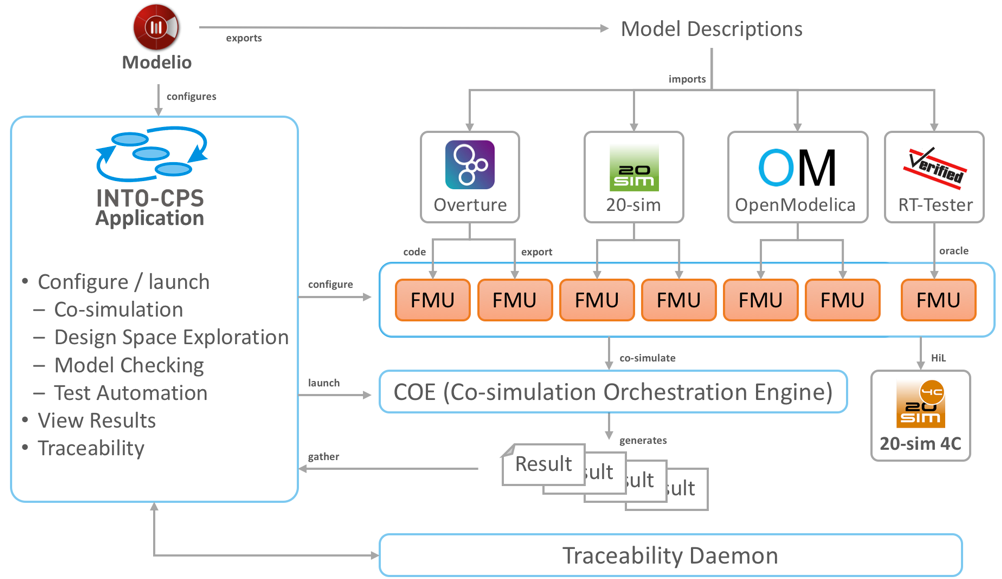
\includegraphics[width=\textwidth]{./figures/toolchain}
\caption{Overview of the INTO-CPS tool chain.}
\label{fig:toolchain}
\end{figure}

The COE connects multiple diverse models, each in the encapsulated form of a Functional Mock-up Unit (FMU) or running in its native modelling environment, to an overall system model. An algorithm for Design Space Exploration (DSE) enables sweeps through ranges of design parameters, performing co-simulations on each. System robustness can be evaluated by using Test Automation (TA) tools that can manipulate the simulation. Links to models can be kept in a database to allow for versioning and traceability even between artefacts produced by different tools. The INTO-CPS tool chain is described in more detail in Section~\ref{sec:toolchain}.
%The entire co-simulation is controlled from a user interface. The final year of the project has seen a significant investment in promoting the co-simulation capabilities, and \url{http://fmi-standard.org/tools/} has been set up as a core webpage for all tools supporting FMI-based co-simulations.

%During Year 3, the COE has been extended with capabilities both for distributed co-simulations and nested co-simulations. A graphical front-end for the entire tool chain called the INTO-CPS Application has been extended considerably. This has been developed further as a desktop application, using web technologies to enable a smoother transition to delivering this as an on-line service should this be desirable in the future . Building on the work of previous years, a 3D FMU support unit has been improved significantly, and has been used for multiple models, including those employed in the industrial case studies.

%Year 3 have seen advances in many other areas of the technology, including new features for Design Space Exploration (DSE), Test Automation (TA), Model Checking (MC), traceability and Code Generation (CG). All of these features have been integrated in the INTO-CPS Application. The final version of the DSE support has been augmented with a capability to deploy DSE on cloud services, making DSE a technology that can be used by businesses without large-scale compute resources of their own. Our SysML profile, designed to ease the high-level development of multi-models, has been extended with features to support disciplined approaches to DSE. The TA and MC capabilities already incorporated in the INTO-CPS Application have been improved during Year 3. Finally, the CG features are incorporated in the different baseline modelling, and simulation tools have been improved in terms of performance and integration. The full deployment of the CG features in a distributed and embedded setting turned out to require more resources than originally envisaged. Most importantly, the support for traceability between different CPS artefacts has been developed during Year 3, including extensions of all the baseline tools with Open Source Life Cycle (OSLC) support. It also turned out that more effort was needed for the full traceability support compared to what was originally envisaged.

\subsection{Case studies}
Inside the INTO-CPS project four industry-led case studies from different application domains have allowed us to evaluate the final INTO-CPS tool chain. These cases (and a couple of industrial cases conducted by external companies) are described further in Section~\ref{sec:casestudies}. A brief overview of the industrial cases inside the INTO-CPS project and their main challenges are:

In the Railways case study led by the French company ClearSy, an innovative distributed interlocking solution has been developed, where signalling safety rules take both the logic and the physical conditions into account with a higher degree of independence than normally. The challenge was to find the right trade-off between the efficiency of an interlocking system (availability of routes, trains' delays and cost of interlocking system) and safety (collision avoidance, derailment prevention, availability and efficiency of the emergency system).

The Agriculture case study led by the Danish company Agrointelli concerns both an automated control system for an agricultural robot as well as an autonomously operating lawn mower. The robot, which provides more efficient removal of weeds in the field while operating safely but with minimal human interaction. In addition, the development of the autonomous control for the lawn mower was carried out. The challenge in both cases was to simulate the behaviour of physical components (such as mechanical loading on certain elements) together with controls of the automated system even before the physical mechanical components are available. These controls access local data (e.g. sensors) and external data (e.g.\ GPS). Model-based design allowed for accelerated time-to-market and virtual verification while reducing the need for multiple physical prototypes. 
%The Year 3 case study also demonstrated that reuse of ideas was possible in the sense that using the INTO-CPS technology development is faster compared to the traditional alternative.

In the Building Automation case study led by the Irish part of United Technology Research Centre (UTRC), CPSs for control of Heating, Ventilation and Air-conditioning (HVAC) have been developed. These CPSs need to be adaptable to components of various manufacturers and different building patterns and the corresponding requirements. The challenge here is also to manage the complexity of the overall system in a way so the co-simulations are sufficiently scalable. The various parts that influence an HVAC system have been modelled and simulated, e.g.\ the fan-coil unit that distributes air, the buildings and rooms as well as the controllers of the fan-coil units. 
%During Year 3 the team has been focusing on evaluating the scalability of the INTO-CPS co-orchestration engine to HVAC models of increased complexity. In the Year 3 use case, the chiller model has been introduced in order to challenge the efficiency and execution of co-simulations using INTO-CPS technology since we have experienced that even commercial tools often fail to deliver the required performance here. 
In addition, UTRC has run an extensive evaluation of all INTO-CPS features including DSE, test automation, Hardware-in-the-Loop (HiL) and 3D co-simulation.   

In the Automotive case study led by the German company TWT, a range optimisation assistant for electric vehicles is being developed. In order to maximise the range without compromising other qualities such as comfort or speed, a comprehensive assessment of the vehicle and its environment is necessary. To achieve this goal, all relevant parts of the system have been modelled, e.g.\ battery, drive train, topography, traffic, weather and cabin thermal control. These constituent models are created in native industrial tools, such as Matlab, and coupled using the INTO-CPS tool suite.

%In Year 3, the final INTO-CPS technologies have been used in all four case studies to get experience with these. 
In order to properly compare the INTO-CPS technology under development with existing modelling and simulation tools, some of the industrial case studies have, on purpose, developed some of their constituent models using such legacy tools (AI has used Gazebo, UTRC has used Dymola and TWT has used Matlab) in order to experiment with the FMUs exported from them in connection with the COE and the rest of the INTO-CPS tool chain. Generally speaking, the results have been quite positive. 
%All four industrial case studies have been extended in different ways (compared to Year 2) and as documented in D1.3a [INTO-CPS-D1.3] progress has been achieved in the assessment of the industrial needs for all four industrial case studies.

\subsection{The INTO-CPS foundations}

The development of tools and methods in INTO-CPS is based on a sound semantic description of co-simulation. Our tools use VDM-RT as the discrete-event language and Modelica as the continuous-time language. The framework for co-simulation is based on FMI. Both languages have been formalised and mechanised in this framework using Isabelle/UTP. We have a semantics of the relevant parts of SysML that can be used with FMI. These foundations allow for the formal checking of the validity of analysis and co-simulation results. There has also been a close integration with the industrial case studies (in particular, the railways and building applications) and supported the development of the INTO-CPS tool chain. It has been demonstrated how to use the foundational tools, with both theorem proving and model checking, to add value to the INTO-CPS tool chain.

\subsection{The INTO-CPS methods and guidelines}

Lowering the barriers to multidisciplinary model-based engineering of CPSs demands methods that permit the deployment of tools in industry processes, embodied in guidelines that reflect experience gained using such methods. We present our modelling methods as guidelines for applying the INTO-CPS tool chain in real industry contexts, with a strong focus on supporting systematic DSE, our form of tradespace analysis, and on managing the traceability of design artefacts. All of the methods and guidelines materials have been made ready for subsequent use by the INTO-CPS Association.  

In order to ease practical deployment of INTO-CPS technology, a SysML profile has been developed to enable designers to move more readily from abstract system models to the structure of heterogeneous co-models. Thus, it has been extended with the ability to help engineers describe explicitly the parameters, objectives and ranking involved in the DSE process, and to allow sweeps to be made both over parameters and operating scenarios. We have developed a Traceability Information Model (TIM) that supports the needs of heterogeneous CPS engineering teams. In defining permissible relations between artefacts and activities, we have drawn on two sources: Open Services for Lifecycle Collaboration (OSLC)  and W3C PROV supported traceability links.

Our guidelines have been implemented in training materials and pilot studies which have been made publicly available and can readily be imported into the INTO-CPS Application, making it easy for newcomers to experiment with the INTO-CPS tools and methods. The pilots provide coverage of all INTO-CPS simulation technologies (VDM-RT, 20-sim and OpenModelica), have architectural models in SysML using the INTO-SysML profile, may be co-simulated with the INTO-CPS Application, can perform DSE, use code generation and have support for test automation. 

\clearpage
%!TEX root = ../INTO-CPS-Manifesto.tex

\newcommand{\CML}{\textsf{CML}}

\section{The INTO-CPS Foundations}\label{sec:foundations}

%\fbox{Jim Woodcock}

%\fbox{JCPW: Add a short introduction}

The development of tools and methods in INTO-CPS is based on a sound semantic description of co-simulation. Our tools use VDM-RT as the discrete-event language and Modelica as the continuous-time language. The framework for co-simulation is based on FMI. We have formalised and mechanised both languages in this framework using Isabelle/UTP. We have a semantics of the relevant parts of SysML that can be used with FMI. These foundations allow for the formal checking of the validity of analysis and co-simulation results. The value of the foundational tools, with both theorem proving and model checking, have been demonstrated to add value to the INTO-CPS tool chain.

\subsection{Foundations of the SysML profile for CPS modelling}

The INTO-CPS project proposes a novel technique for proof-based analysis of co-simulations that considers both architectural and behavioural properties of co-simulations. In D2.3a~\cite{INTO-CPS-D2.3a-2017}, the technique is illustrated by way of two case studies, one from from railways and another one from the area of smart buildings control. D2.2a~\cite{INTO-CPS-D2.2a-2016} instantiates the approach to robotic control.

\subsubsection{SysML}

The Systems Modelling Language (SysML)~\cite{OMGSysML2012} builds on the Unified Modelling Language (UML) to provide a general-purpose notation for systems engineering. SysML supports the modelling of CPSs, which are designed to actively engage with the physical world in which they reside. They tend to be heterogeneous: their subsystems tackle a wide variety of domains (such as, mechanical, hydraulic, analogue, and a plethora of software domains) that mix phenomena of both continuous and discrete nature, typical of physical and software systems, respectively. Such systems are typically engineered using a variety of languages and tools that adopt complementary paradigms; examples are physics-related models, control laws, and sequential, concurrent, and real-time programs. This diversity makes CPS generally difficult to analyse and study.

\subsubsection{Co-simulation}

CPSs are often handled modularly to tackle this heterogeneity and complexity. To separate concerns effectively, the global model of the system is decomposed into subsystems, each typically focused on a particular phenomenon or domain and tackled by the most appropriate modelling technique. Simulation, the standard validation technique for CPS, is often carried out modularly also, using co-simulation~\cite{GomesTBLV2017,Gomes&18}, the coupling of subsystem simulations. This constitutes the backdrop of the industrial Functional Mockup Interface (FMI) standard~\cite{FMIStandard2014,BromanBGLMTW2013,CavalcantiWA16} for co-simulation of components built using distinct modelling tools. The FMI Standard has been proposed to address the challenge of interoperability, coupling different simulators and their high-level control components via a bespoke FMI API.

While co-simulation is currently the predominant approach to analyse CPS, INTO-CPS proposes a proof-based complementary technique that uses mathematical reasoning and logic. Simulation is useful in helping engineers to understand modelling implications and spot design issues, but cannot provide universal guarantees of correctness and safety. It is usually impossible to run an exhaustive number of simulations as a way of testing the system. For these reasons, it is often not clear how the evidence provided by simulations is to be qualified, since simulations depend on parameters and algorithms, and are software systems (with possible faults) in their own right.

Proof-based techniques, on the other hand, hold the promise of making universal claims about systems. They can potentially abstract from particular simulation scenarios, parametrisations of models, and interaction patterns used for testing. In traditional software engineering, they have been successfully used to validate the correctness of implementations against abstract requirements models~\cite{WoodcockLBF2009}. Yet, their application to CPS is fraught with difficulties: the heterogeneous combination of languages used in typical descriptions of CPS raises issues of semantic integration and complexity in reasoning about those models. The aspiring ideal of any verification technique is a compositional approach, and such approaches are still rare for CPS~\cite{NuzzoLFS2018}.

\subsubsection{The INTO-CPS approach to verification and co-simulation}

Our approach is to formally verify the well-formedness and healthiness of SysML CPS architectural designs as a prelude to co-simulation. The designs are described using INTO-SysML~\cite{INTO-CPS-D2.1a-2015}, a profile for multi-modelling and FMI co-simulation. The well-formedness checks verify that designs comply with all the required constraints of the INTO-SysML meta-model; this includes connector conformity, which checks the adequacy of the connections between SysML blocks (denoting components) with respect to the types of the ports being wired. The healthiness checks concern detection of algebraic loops, a feedback loop resulting in instantaneous cyclic dependencies; this is relevant because a desirable property of co-simulation, which often reduces to coupling of simulators, is convergence (where numerical analyses approximate the solution), which is dependent on the structure of the subsystems and cannot be guaranteed if this structure contains algebraic loops~\cite{KublerS2000,BromanBGLMTW2013}. The work in the INTO-CPS project demonstrates the capabilities of our verification workbench for modelling languages and engineering theories mechanised in the Isabelle proof assistant~\cite{NipkowK2014}, and the CSP process algebra~\cite{Hoare1985} with its accompanying FDR3 refinement-checker~\cite{GibsonRobinsonABR2016}.

Our technique is based on abstraction: we use a relational view of FMUs that abstracts from reactive behaviours as well as the API imposed by FMI. This allows us to focus on the fundamental properties of a co-simulation, while introducing details into the model view refinement that preserves those properties.

\subsubsection{Instantiation for robotics applications}

We have extended and restricted the INTO-SysML profile to deal with mobile and autonomous robotic systems. For modelling the controllers, we use RoboChart~\cite{LiMRCWT2017}. For modelling the robotic platform and the environment, we use Simulink~\cite{MathworksURL}. We have also given a behavioural semantics for models written in the profile using CSP. The semantics is agnostic to RoboChart and Simulink, and captures a co-simulation view of the multi-models based on the FMI API.

Our semantics can be used in two ways. First, by integration with a semantics of each of the multi-models that defines their specific responses to the simulation steps, we can obtain a semantics of the system as a whole. Such semantics can be used to establish properties of the system, as opposed to properties of the individual models. In this way, we can confirm the results of co-simulations via model checking or theorem proving, for example.

There are CSP-based formal semantics for RoboChart~\cite{MiyazawaCRLWT2016} and Simu\-link~\cite{MarriottZC2012,CavalcantiMW2013} underpinned by a precise mathematical semantics. Our next step is their lifting to provide an FMI-based view of the behaviour of models written in these notations. With that, we can use RoboChart and Simulink models as FMUs in a formal model of a co-simulation as suggested here, and use CSP and its semantics to reason about the co-simulation.

It is also relatively direct to wrap existing CSP semantics for UML state machines~\cite{DaviesC2003,RaschW2005} to allow the use of such models as FMUs in a co-simulation. In this case, traditional UML modelling can be adopted.

Secondly, we can use our semantics as a specification for a co-simulation. The work in~\cite{CavalcantiWA16} provides a CSP semantics for an FMI co-simulation; it covers not only models of the FMUs, but also a model of a master algorithm of choice. The scenario defined by an INTO-SysML model identifies inputs and outputs, and their connections. The traces of the FMI co-simulation model should be allowed by the CSP semantics of the INTO-SysML model.

There is no support to establish formal connections between a simulation and the state machine and physical models (of the robotic platform and the environment). The SysML profile proposed here supports the development of design models via the provision of domain-specific languages based on familiar diagrammatic notations and facilities for clear connection of models. Complementarily, as explained above, the semantics of the profile supports the verification of FMI-based co-simulations.  There are plans for automatic generation of simulations of RoboChart models~\cite{CavalcantiWA16}. The semantics we propose can be used to justify the combination of these simulations with Simulink simulations as suggested above.

\subsubsection{Future work}

We first suggest the development of a tool that supports the user of our technique in automatically generating the Isabelle/UTP architectural model, as well as a sketch of the behavioural model. The formal developer can use the sketch as a starting point, completing it with a detailed encoding of functional behaviours of FMUs. Secondly, elements of the refinement strategy from abstract into concrete FMU models ought be explored for a larger spectrum of case studies and examples, beyond the ones we presented in this report. Both these works could be tackled by the INTO-CPS Association.

INTO-CPS multi-models are composed of individual models whose foundations lie in a variety of modelling notations, each of which has its own unique syntax, semantics, and underlying paradigmatic concepts, such as discrete or continuous time.  The purpose of a multi-model is to assign behaviour to a CPS by composing the behaviours of the constituent models.  Thus, in order to provide an integrated tool chain for trustworthy CPS development, there is a necessity for unification of these underlying semantic models to allow consistent integration of heterogeneous system components.  This will then allow us to substantiate statements made about the multi-model with respect to the underlying mathematical core.  Hoare and He's UTP~\cite{Hoare&98} has been designed as a framework in which the integration of languages, through the common semantic domain of the alphabetised relation calculus, can be achieved.  In the next two sections, we describe how UTP is used to provide the foundations for continuous-time modelling in the INTO-CPS tool chain.

\subsection{Discrete Event Models}

VDM-RT is a real-time dialect of the VDM formal modelling language that can be applied to the specification of discrete controllers for CPSs.  VDM-RT is object oriented, where all models are defined as classes that are instantiated as objects.  It supports concurrency through threading and communication between threads through shared objects.  The real-time features of the language comprise abstractions for deployment of objects to computing units that are connected by buses, and the time taken to evaluate expressions that advance a global ``wall clock'' to predict the computation time of a model.

A denotational semantics exists for the core specification language~\cite{Larsen&95c}, and a structured operational semantics (SOS) exists for the real-time aspects~\cite{Lausdahl&13a}, but there is currently no full semantic description of VDM-RT.  To address this, the INTO-CPS project has established a comprehensive denotational semantics for the VDM-RT language, including object orientation, real time, and concurrency.

We have given a UTP semantics to the language, and mechanised this in the Isabelle/UTP theorem prover.  The basis for our treatment of object orientation is an extended calculus for classes and objects, including novel healthiness conditions that allow handling of multiple inheritance.  Our semantics includes a new approach to handling static attributes, methods, and constructors.  We have mechanised Lausdahl's operational semantics of VDM-RT~\cite{Lausdahl&13a} in Isabelle/HOL, which allowed us to gain greater insight into the language.

We use UTP~\cite{Hoare&98,Cavalcanti&06} to give a denotational semantics to VDM-RT.  VDM-RT is a discrete real-time language, which leads us to employ the UTP theory of timed reactive designs as the semantic model, as embodied in the COMPASS Modelling Language (\CML) \cite{Woodcock&12a,Woodcock14,Woodcock&14}.  We use the constructs of \CML\ to describe VDM-RT objects, threads, CPUs, and busses, together with actions that encode their orchestrated execution.  In order to accomplish this, we also extend \CML\ with a universe type for VDM-RT, and also timed expressions that cause language constructs like assignment to expend time during execution.

Our semantics of VDM-RT is based on a pattern commonly employed in the INTO-CPS project to describe the discrete time component of a CPS.  Such a ``cyber component'' consists of one or more controller objects, each of which owns a number of sensors and actuators through which to interact with the physical components.  The topology of such a cyber component is thus fixed at instantiation, and there is no necessity to support dynamic object creation, which thus favours the use of static \CML\ processes to represent objects and threads.  Limiting ourselves to static topologies enables the application of static analysis techniques like model checking~\cite{fdr,Oliveira2014,Beg2015}, which typically requires a tractable state space.

\subsection{Continuous Models}

Modelling of continuous dynamical systems in the INTO-CPS tool chain is provided by the Modelica and 20-sim tools, both of which are based on differential equations.  We have created a formal denotational semantics for continuous-time models written using the Modelica language~\cite{ModelicaAssociation2014}.  The creation of such a semantics provides firm mathematical foundations for the language, allowing us to consider formal links between Modelica and other languages in INTO-CPS, and enabling theorem-proving support for continuous models.  The Modelica language supports modelling based on ordinary differential equations (ODEs) and differential algebraic equations (DAEs) combined with an event handling mechanism.

We have provided a \emph{flattening} process, whereby a collection of Modelica objects is converted to a pure hybrid DAE system, the core of the Modelica language. In our work, we have compared this to the FMI representation of Hybrid ODEs.  Once more, we have used the UTP semantic framework~\cite{Hoare&98} to give Modelica a formal semantics, along with other continuous time and dynamical systems modelling languages.  Our theory of differential algebraic equations allows the definition of hybrid programs that mix continuous and discrete behaviour, and also specifications regarding their behaviour.

We have mechanised our UTP theory in the established Isabelle/HOL proof assistant~\cite{Isabelle}.  This allowed us to also show that our calculus satisfies well-known laws of programming.  Our combination of continuous invariants with timed reactive designs~\cite{Hayes2010,Canham15}, forms the basis of a refinement technique for hybrid systems.

Our hybrid combination of discrete and continuous models is known as \CyPhyCircus.  We have defined mappings from the core languages in \CyPhyCircus which, as illustrated Figure~\ref{fig:CyPhyCircus}, will also enable access to a number of static analysis tools and techniques, such as model checking~\cite{Oliveira2014,Beg2015,Beg2016} and theorem proving~\cite{Foster14,Foster16a,Zeyda16}.  \CyPhyCircus build on the existing work of the \Circus language family~\cite{Woodcock&01,OCW2007,Woodcock14}, a suite of formal languages that combines rich state modelling (like as in the Z specification language~\cite{Woodcock&96}) with concurrency (as in CSP~\cite{Hoare1985}), with various other programming paradigms such as object orientation~\cite{Cavalcanti2005} and discrete real-time modelling~\cite{Wei2013}.  The intention is to have a language that combines rich-state modelling, concurrent reactive processes, real-time modelling, continuous variables, and differential equations.  The theory of hybrid relations provides the foundations for such hybrid dynamical behaviour in \CyPhyCircus.

\begin{figure}
  \begin{center}
    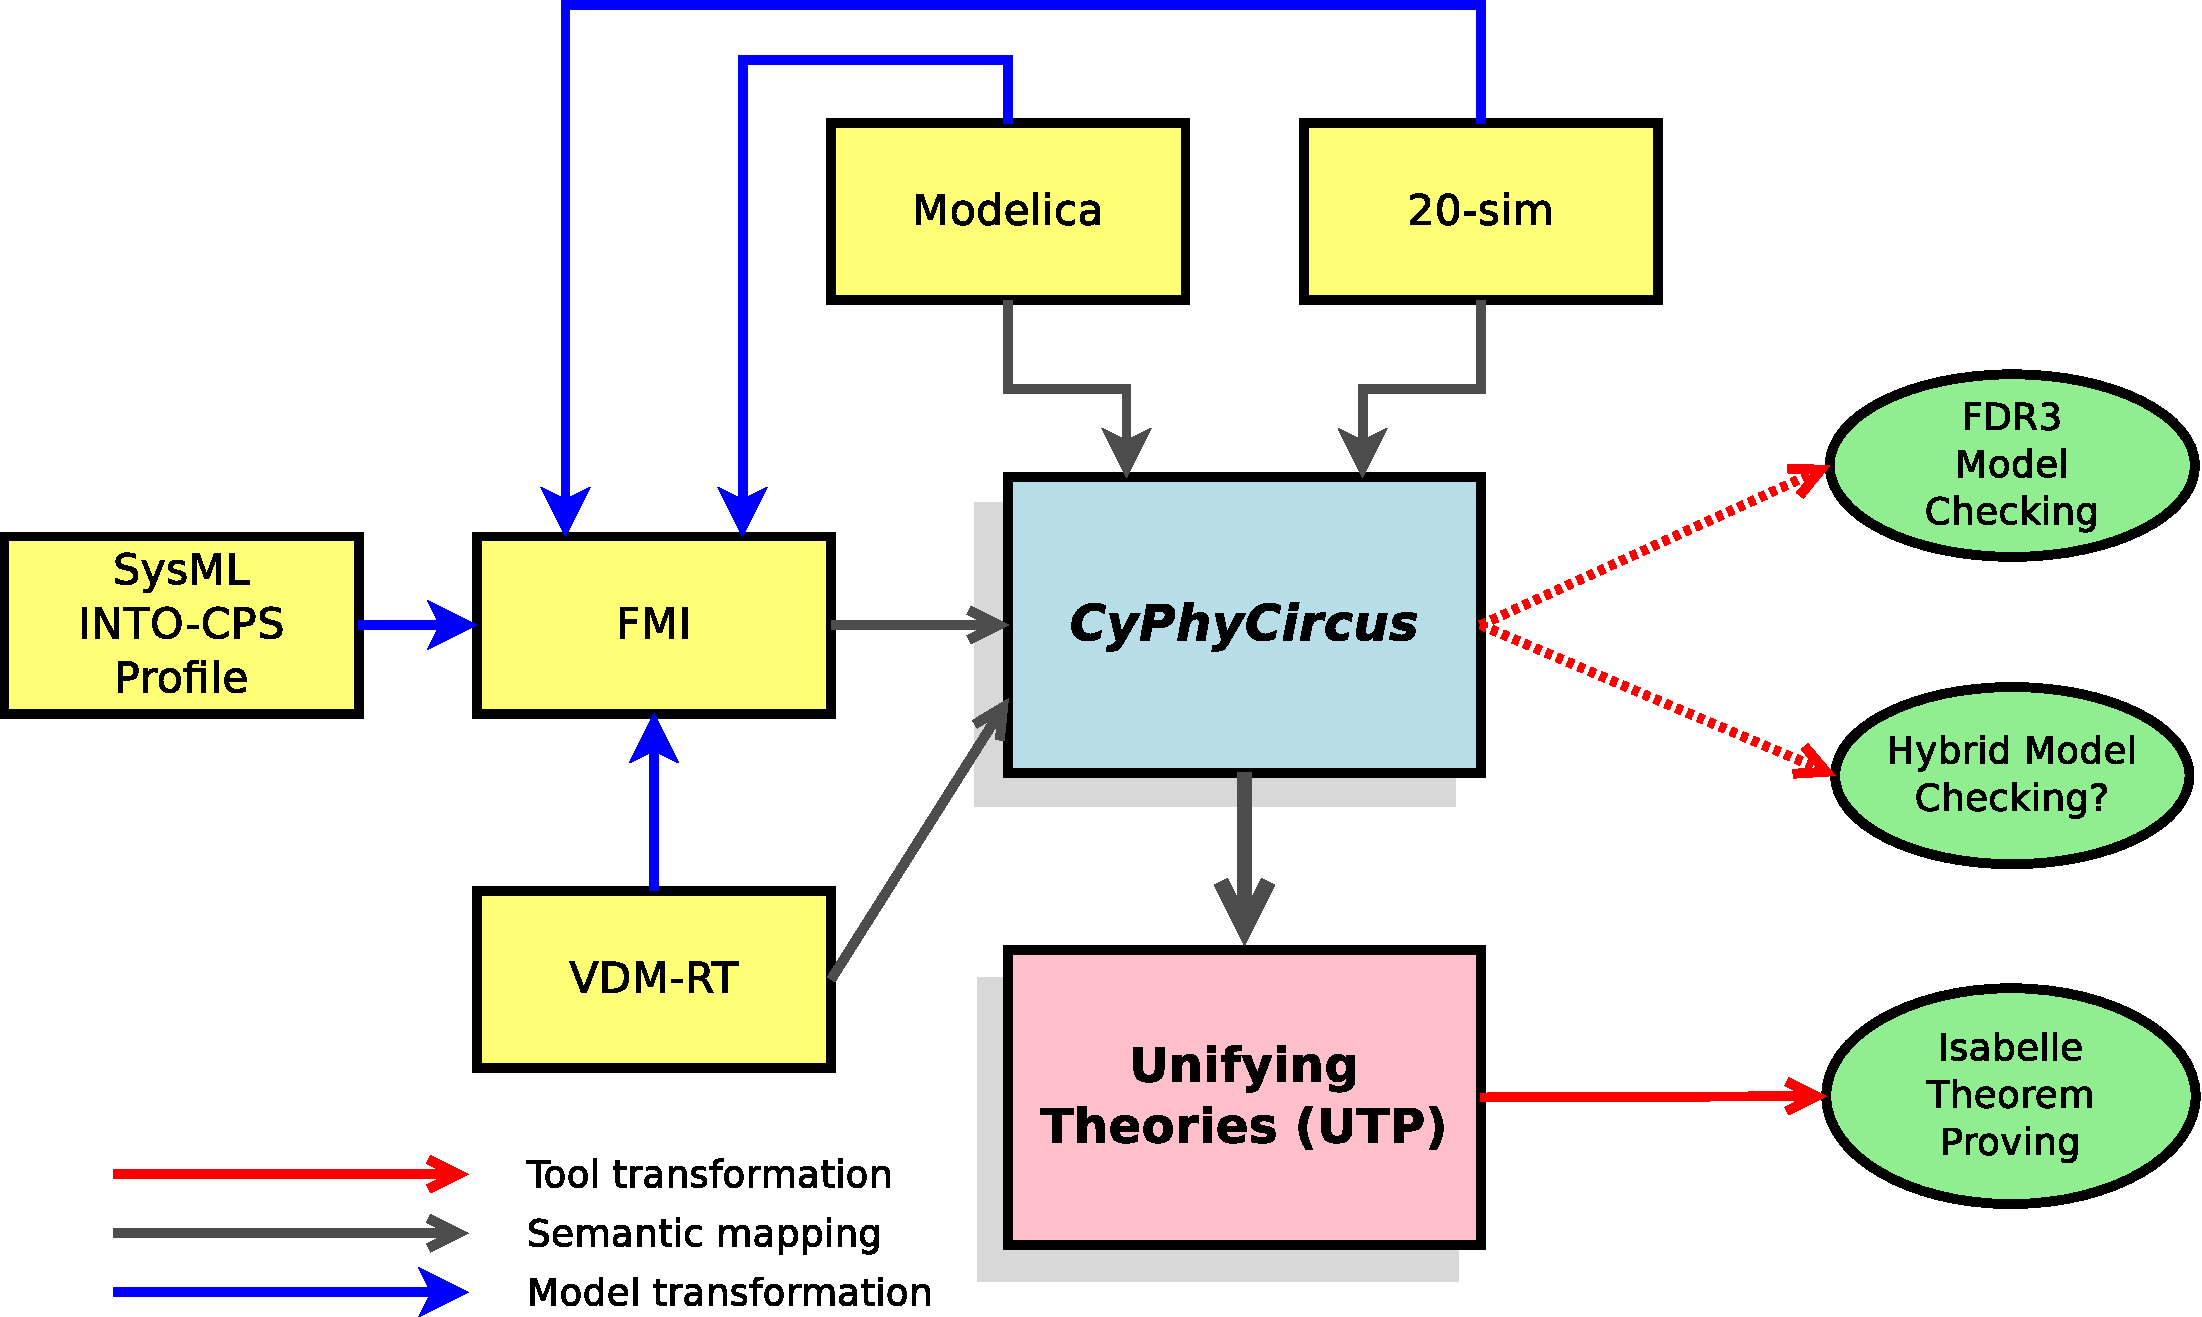
\includegraphics[width=14cm]{CyPhyCircus}
  \end{center}
  \caption{\CyPhyCircus as the INTO-CPS lingua franca}
  \label{fig:CyPhyCircus}
\end{figure}

\subsection{Functional Mock-up Interface}%

Because CPSs comprise both real-world entities and digital components, their modelling and designing typically requires a combination of different languages and tools that adopt complementary specification paradigms. For real-world artefacts, physics models in the form of differential equations are the norm. Digital components, such as software controllers, are typically described via control diagrams, state machines, and real-time programs. This diversity of specification and design methods makes CPS challenging to study and analyse.

Cosimulation~\cite{GomesTBLV2017} is perhaps the de facto technique for analysing the behaviour of CPS. It requires that models of artefacts are simulated in isolation, while master algorithms control the various simulators and thereby orchestrate the cosimulation as a whole. This raises issues of interoperability between the master algorithm and the simulators. The Functional Mock-up Interface (FMI) Standard~\cite{Blochwitz2011} has been proposed to alleviate those issues, and has since been successfully used in many industrial applications.  The FMI standard prescribes how master algorithms (MA) and simulators communicate. It does so using a bespoke API that simulators have to implement, and that can be used to devise compliant master algorithms. The API enables master algorithms to exchange data between the components of a cosimulation, called FMUs (Functional Mock-up Units), perform simulation steps, and suitably deal with errors in simulators. It also allows for advanced features such as roll-back of already performed steps.

While (co)simulation is currently the predominant approach to validate CPS models, the INTO-CPS approach uses a complementary technique based on a formal model of an FMI system. Our technique formalises both the master algorithm and the simulated FMUs, and allows for verification of their properties.

Whereas (co)simulation helps engineers to quickly gauge the implications of modelling and design decisions, our formal analysis has the potential to complement simulation with universal guarantees, both about the master algorithm and cosimulated system. The former is important since simulations depend on parameters and algorithms, and are software systems (with possible faults) in their own right. The latter is important since it is usually not possible to run an exhaustive number of simulation scenarios as a means of testing the system towards producing strong certification evidence.

For our formal modelling, we use Circus: a process algebra with added features for supporting stateful models. It has proved adequate and useful for modelling master algorithms~\cite{CavalcantiWA16} due to its capabilities of capturing concisely the data and control aspects of such algorithms, including data exchange between the FMUs and their concurrent execution. Circus models can be subjected to verification techniques. These include both model-checking approaches~\cite{GrumbergV2008}, refinement~\cite{CavalcantiSW2003}, and (automatic) theorem proving~\cite{OliveiraCW2009}.

We use an abstract relational model of FMI cosimulations that focuses on the essence of the FMI computational paradigm~\cite{ZCWO17}. We have considered a concrete reactive model of FMI that faithfully models the FMI interface as well as master algorithms. This extends and elaborates our previous work by providing a comprehensive Circus model that has been mechanised in the theorem prover Isabelle/UTP~\cite{FosterZW2016}.

We have presented a complete and final Circus model of the FMI standard for cosimulation. To accomplish this, we have embedded the Circus language into Isabelle/UTP, allowing us to mechanise our FMI Circus model.  We illustrated the use of our mechanisation by applying it to one of the industrial INTO-CPS case studies (a railways system).

For proof support, we pursue a technique, based on refinement, to show compliance of master algorithms with regards to the FMI standard~cite{FMI2014}. Unlike other approaches, such as~\cite{Broman2013}, we can profit from high-level algebraic laws and a stepwise approach that culminates in executable code, for both the FMUs and master algorithm.

We have shown how our work completes the general reasoning technique. That technique proposes a refinement-based approach: we start with a discrete abstraction of a cosimulation that does not need to consider the master algorithm and is used to establish fundamental safety properties. Our work has filled an important gap: the transformation of an abstract FMU model into a concrete one that can be translated into code.
\clearpage
\section{INTO-CPS Method Guidelines}
\label{sec:method}

\subsection{Introduction}
\label{sec:method:intro}

The INTO-CPS tool chain enables collaborative multidisciplinary model-based design of CPSs. Although each discipline involved in a CPS engineering enterprise has its own culture, abstractions, and approaches to problem solving, it may only be on federating them that knowledge which is otherwise tacit in some disciplines has to be made explicit. To date, there is only limited experience in model-based multidisciplinary design of CPSs, and so the methods and approaches for bringing models together are only beginning to emerge. This section aims to distil the methods and guidelines that have emerged in our experience with the INTO-CPS toolchain, and to do so in a way that helps the reader understand how best to use INTO-CPS co-modelling technologies.

This section complements the Tool Chain User Manual~\cite{INTOCPSD4.3a}--- which gives detail on how to use the features of the tool chain--- by providing guidance on when and why you might use these features. The guidance given here has been distilled from experience gained through pilot studies and applications of INTO-CPS technologies to real industrial cases. These pilot studies now appear as examples that can be opened directly from the INTO-CPS Application, supported by descriptions in the Examples Compendium~\cite{INTOCPSD3.6}. Industrial applications are described in the Case Studies report~\cite{INTOCPSD1.3a}. Sections~\ref{sec:method:intro}--\ref{sec:method:workflows} provide an introduction to core INTO-CPS terminology and the activities that INTO-CPS enables. Advanced topics including traceability, design space exploration, architectural modelling, New users are recommended to:

%\begin{itemize}[noitemsep]
\begin{itemize}
  \item Read the introductory material in Sections~\ref{sec:method:intro}--\ref{sec:method:workflows}.
  \item Follow the first tutorial to experience the INTO-CPS Application.
  \item Import one or two examples from the Examples Compendium\footnote{\url{https://github.com/INTO-CPS-Association/training/tree/master/tutorials}} into the INTO-CPS Application and interact with them.
  \item As you start your own multi-modelling, return to this section for guidance on particular topics as required.
\end{itemize}

\subsection{Concepts and Terminology}
\label{sec:method:concepts}

Given the diversity of backgrounds in CPS engineering teams, it is worth clarifying some common concepts.

\subsubsection{Systems}
\label{sec:concepts:systems}
A \term{System} is ``a combination of interacting elements organized to achieve one or more stated purposes''~\cite{INCOSEseh15}. Any given system will have an~\term{environment}, considered to be everything outside of the system. The behaviour exhibited by the environment is beyond the direct control of the developer~\cite{Broenink&12b}. A \term{system boundary} is the common frontier between a system of interest and its environment~\cite{Broenink&12b}. An \term{interface} is a shared boundary between two entities, which can be defined in terms of physical and digital interactions and flows~\cite{INCOSEseh15}.


\term{Cyber-Physical Systems (CPSs)} are ``ICT systems (sensing, actuating, computing, communication, etc.) embedded in physical objects, interconnected (including through the Internet) and providing citizens and businesses with a wide range of innovative applications and services''~\cite{Thompson13, Deka&15}.

Many CPSs are \term{Systems of Systems (SoSs)}. An SoS is a ``collection of independent systems, integrated into a larger system that delivers unique capabilities''~\cite{INCOSEsosprimer18}.
%Many CPSs are \term{Systems of Systems (SoSs)}. An SoS is a ``collection of constituent systems that pool their resources and capabilities together to create a new, more complex system which offers more functionality and performance than simply the sum of the constituent systems''~\cite{Holt&14}. CPSs may exhibit the characteristics of SoSs.

\subsubsection{Models}
\label{sec:concepts:models}

A \term{model} is a  potentially partial and abstract description of a system, limited to those components and properties of the system that pertain to the current goal~\cite{Holt&14}. A model should be ``just complex enough to describe or study the phenomena that are relevant for our problem context''~\cite{Amerongen10}. Models should be abstract ``in the sense that aspects of the product not relevant to the analysis in hand are not included''~\cite{Fitzgerald&98b}. A model ``may contain representations of the system, environment and stimuli''~\cite{Fitzgerald&14c}

%\fbox{Further discussion may be required on the definition of: environment models, test models in RT-Tester and their correspondence in the INTO-CPS SysML profile?}.

In a CPS model, we describe systems with cyber, physical and network elements. These components are often modelled in a variety of languages, with different notations, concepts, levels of abstraction, and semantics, which are not necessarily easily mapped one to another. We use \term{continuous time (CT)} and \term{discrete event (DE)} models to represent physical and cyber elements as appropriate. A CT model has state that can be changed and observed \emph{continuously}~\cite{Amerongen10} and is described using either explicit continuous functions of time or implicitly as a solution of differential equations. A DE model has state that can be changed and observed only at fixed, \emph{discrete}, time intervals~\cite{Amerongen10}.  We use the term \term{multi-model} to refer to the federation of several constituent DE and CT models.

A \term{requirement} may impose restrictions, define capabilities or identify qualities of a system, and should indicate some value or use for the stakeholders in a CPS. \term{Requirements Engineering (RE)} is the process of specifying and documenting requirements placed upon a CPS. Requirements may be considered in relation to different \term{contexts} -- that is the point of view of some system component or domain, or interested stakeholder.

A \term{design parameter} is a property of a model that can be used to affect the model's behaviour, but remains constant during a given simulation~\cite{Broenink&12b}. A \term{variable} is feature of a model that may change during a given simulation~\cite{Broenink&12b}. \term{Non-functional properties (NFPs)} pertain to characteristics other than functional correctness. For example, reliability, availability, safety and performance of specific functions or services are NFPs that are quantifiable. Other NFPs may be more difficult to measure~\cite{Payne&10}.

The activity of creating models may be referred to as \term{modelling} ~\cite{Fitzgerald&14c} and related terms include \term{co-modelling} and \term{multi-modelling}. A \term{workflow} is a sequence of \term{activities} performed to aid in modelling. A workflow has a defined purpose, and may cover a subset of the CPS engineering development lifecycle.

The term \term{architecture} has many different definitions, and range in scope depending upon the scale of the product being `architected'. We use the simple definition from~\cite{COMPASSD22.6}:  ``an architecture defines the major elements of a system, identifies the relationships and interactions between the elements and takes into account process. Those elements are referred to as \term{components}. An architecture involves both a definition of structure and behaviour. Importantly, architectures are not static but must evolve over time to reflect the change in a system as it evolves to meet changes to its requirements''. In a CPS architecture, components may be either \term{cyber components} or \term{physical components} is they describe computational or physical elements.

We consider both \term{holistic} and a \term{design} architectures~(Section~\ref{sec:method:sysml}). The aim of a holistic architecture is to identify the units of functionality of the system reflecting the \emph{terminology and structure of the domain of application}. It describes a conceptual model of these units and their interconnections, giving a holistic view of the overall system. The design architectural model of the system is effectively a multi-model. The INTO-CPS SysML profile~\cite{INTOCPSD2.1a} is designed to assist in the specification of CPS design architectures. It helps the architect describe a system as a decomposition into interconnected \term{subsystems}, each of which is an assembly of cyber and physical components and possibly other subsystems. Each of these components and subsystems can be modelled separately in a domain-specific notation and tool.

\term{Evolution} refers to the ability of a system to benefit from a varying number of alternative system components and relations, as well as its ability to gain from the adjustments of the individual components' capabilities over time.
%An \term{interface} defines the boundary across which two entities meet and communicate with each other~\cite{Holt&14}. Interfaces may describe both digital and physical interactions: digital interfaces  contain descriptions of operations and attributes that are \emph{provided} and \emph{required} by components. Physical interfaces describe the flow of physical matter (for example fluid and electrical power) between components.

There are many methods of describing architectures. An \term{architecture diagram} is a symbolic representation of architectural information contained in a model. An \term{architectural framework} is a ``defined set of viewpoints and an ontology'' and ``is used to structure an architecture from the point of view of a specific industry, stakeholder role set, or organisation. In the application of an architecture framework, an \term{architectural view} is a ``work product (for example an architecture diagram) expressing the architecture of a system from the perspective of specific system concerns''~\cite{COMPASSD22.6}.

The \into\ SysML profile comprises diagrams for architectural modelling and specifying \term{design space exploration}. There are two architectural diagrams. The \term{Architecture Structure Diagram (ASD)} specialises SysML block definition diagrams to support the specification of a system architecture described in terms of a system's components. \term{Connections Diagrams (CDs)} specialise SysML internal block diagrams to convey the internal configuration of the system's components and the way they are connected. The system architecture defined in the profile should inform a co-simulation multi-model and therefore all components interact through connections between flow ports. The profile permits the specification of \term{cyber} and \term{physical} components and also components representing the \term{environment} and \term{visualisation} elements. The \into\ SysML profile includes three design space exploration diagrams: a \term{parameters diagram}; an \term{objective diagram}; and a \term{ranking diagram}. See Section~\ref{sec:concepts:analysis} for concepts relating to design space exploration.


\subsubsection{Tools}
\label{sec:concepts:tools}

The \term{\into\ tool chain} is a collection of software tools, based centrally around FMI-compatible co-simulation, that  supports the collaborative development of CPSs. The \term{\into\ Application} is a front-end to the INTO-CPS tool chain. The Application allows the specification of the co-simulation configuration, and the co-simulation execution itself. The application also provides access to features of the tool chain without an existing user interface (such as design space exploration and model checking).

Central to the \into\ tool chain is the use of the \term{Functional Mockup Interface (FMI)} standard. This is a tool-independent standard to support both model exchange and co-simulation of dynamic models using a combination of XML-files and compiled C-code~\cite{FMIStandard2.0}. Part of the FMI standard for model exchange is specification of a \term{model description} file. This is an XML file that supplies a description of all properties of a model (for example input/output variables). A \term{Functional Mockup Unit (FMU)} is a tool component that implements FMI. Data exchange between FMUs and the synchronisation of all simulation solvers~\cite{FMIStandard2.0} is controlled by a \term{Master Algorithm}.

\term{Co-simulation}  is the simultaneous, collaborative, execution of models and allowing information to be shared between them. The models may be CT-only, DE-only or a combination of both. The \term{Co-simulation Orchestration Engine (COE)} combines existing co-simulation solutions (FMUs) and scales them to the CPS level, allowing CPS multi-models to be evaluated through co-simulation. This means that the COE implements a \term{Master Algorithm}. The COE will also allow real software and physical elements to participate in co-simulation alongside models, enabling both Hardware-in-the-Loop (HiL) and Software-in-the-Loop (SiL) simulation.

In the \into\ Application, a \term{project} comprises: a number of FMUs, optional source models (from which FMUs are exported); a collection of \term{multi-models}; and an optional SysML architectural model. A multi-model includes a list of FMUs, defined instances of those FMUs, specified connections between the inputs/outputs of the FMU instances, and defined values for design parameters of the FMU instances. For each multi-model a \term{co-simulation configuration} defines the step size configuration, start and end time for the co-simulation of that multi-model. Several configurations can be defined for each multi-model.

\term{Code generation} is the transformation of a model into generated code suitable for compilation into one or more target languages (e.g. C or Java).

We consider two tool-supported methods for recording the rationale of design decisions in CPSs.  \term{Traceability} is the association of one model element (e.g., requirements, design artefacts, activities, software code or hardware) to another. \term{Requirements traceability} ``refers to the ability to describe and follow the life of a requirement, in both a forwards and backwards direction''~\cite{Gotel&94}. \term{Provenance} ``is information about entities, activities, and people involved in producing a piece of data or thing, which can be used to form assessments about its quality, reliability or trustworthiness'' ~\cite{Moreau&13}. In \into\ traceability between model elements defined in the various modelling tools is achieved through the use of \term{OSLC messages}, handled by a traceability \term{daemon tool}. This supports the \term{impact analysis} and general \term{traceability queries}.

Two broad groups of users are considered in the \into\ project. A \term{Tool Chain User} is an individual who uses the \into\ Tool Chain and its various analysis features. A \term{Foundations Developer} is someone who uses the developed foundations and associated tool support (see Section~\ref{sec:concepts:formal}) to reason about the development of tools.

\subsubsection{Analysis}
\label{sec:concepts:analysis}

\term{Design-Space Exploration (DSE)} is ``an activity undertaken by one or more engineers in which they build and evaluate [multi]-models in order to reach a design from a set of requirements''~\cite{Broenink&12b}. ``The \term{design space} is the set of possible solutions for a given design problem''~\cite{Broenink&12b}. Where two or more models represent different possible solutions to the same problem, these are considered to be \term{design alternatives}. In \into\, design alternatives are defined using either a range of parameter values or different multi-models. Each choice involves making a selection from alternatives on the basis of an \term{objective} -- criteria or constraints that are important to the developer, such as cost or performance. The alternative selected at each point constrains the range of design alternatives that may be viable next steps forward from the current position. Given a collection of alternatives with corresponding objective results, a \term{ranking} may be applied to determine the `best' design alternative.

\term{Test Automation (TA)} is defined as the machine assisted automation of system tests. In \into, we concentrate on various forms of \term{model-based testing} -- centering on testing system models, against the requirements on the system. The \term{System Under Test (SUT)} is ``the system currently being tested for correct behaviour. An alias for system of interest, from the point of view of the tester''~\cite{Holt&14}. The SUT is tested against a collection of \term{test cases} --  a finite structure of input and expected output~\cite{Utting&06}, alongside a \term{test model}, which specifies the expected behaviour of a system under test~\cite{Coleman&13b}. TA uses a \term{test suite} -- a collection of \term{test procedures}. These test procedures are detailed instructions for the set-up and execution of a given set of test cases, and instructions for the evaluation of results of executing the test cases~\cite{DO178B}.

\into\ considers three main types of test automation: \term{Hardware-in-the-Loop (HiL)}, \term{Software-in-the-Loop (SiL)} and \term{Model-in-the-Loop (MiL)}. In \term{HiL} there is (target) hardware involved, thus the FMU is mainly a wrapper that interacts (timed) with this hardware; it is perceivable that realisation heavily depends on hardware interfaces and timing properties.
%testing with DE models running on target hardware components;
In \term{Software-in-the-Loop (SiL)} testing the object of the test execution is an FMU that contains a software implementation of (parts of) the system. It can be compiled and run on the same machine that the COE runs on and has no (defined) interaction other than the FMU-interface.
%    It does not matter (much) where this implementation comes from.
%testing with software running on CT model simulator;
Finally, in \term{Model-in-the-Loop (MiL)} the test object of the test execution is a (design) model, represented by one or more FMUs. This is similar to the SiL (if e.g., the SUT is generated from the design model), but MiL can also imply that running the SUT-FMU has a representation on model level; e.g., a playback functionality in the modelling tool could some day be used to visualise a test run.
%testing with co-simulated CT/DE models. \fbox{Check definitions}

\term{Model Checking (MC)} exhaustively checks whether the model of the system meets its specification~\cite{Clarke&99}, which is typically expressed in some temporal logic such as \term{Linear Time Logic (LTL)}~\cite{Pnueli77} or \term{Computation Tree Logic (CTL)}~\cite{Clarke&81}. As opposed to testing, model checking examines the entire state space of the system and is thus able to provide a correctness proof for the model with respect to its specification. In INTO-CPS, we can concentrate on \term{Bounded Model Checking (BMC)}~\cite{Clarke&01,Clarke&04,Clarke&05}, which is based on encodings of the system in propositional logic, for a timed variant of LTL. The key idea of this approach is to represent the semantics of the model as a Boolean formula and then apply a \term{Satisfiability Modulo Theory (SMT)}~\cite{Kroening&08} solver in order to check whether the model satisfies its specification. A powerful feature of model checking is that, if the specification is violated, it provides a counterexample trace that shows exactly how an undesired state of the system can be reached~\cite{Clarke&03}.

\subsubsection{Existing Tools and Languages}
\label{sec:concepts:language}

The \into\ tool chain uses several existing modelling tools. \term{Overture}\footnote{\url{http://overturetool.org/}} supports modelling and analysis in the design of discrete, typically, computer-based systems using the \term{VDM-RT} notation. VDM-RT is based upon the \term{object-oriented} paradigm where a model is comprised of one or more \term{objects}. An object is an instance of a \term{class} where a class gives a definition of zero or more \term{instance variables} and \term{operations} an object will contain. Instance variables define the identifiers and types of the data stored within an object, while operations define the behaviours of the object.

The \term{20-sim}\footnote{\url{http://www.20sim.com/}} tool can represent continuous time models in a number of ways. The core concept is that of connected \term{blocks}.   \term{Bond graphs} may implement blocks. Bond graphs offer a domain-independent description of a physical system's dynamics, realised as a directed graph. The vertices of these graphs are idealised descriptions of physical phenomena, with their edges (\term{bonds}) describing energy exchange between vertices. Blocks may have input and output \term{ports} that allow data to be passed between them. The energy exchanged in 20-sim is the product of \term{effort} and \term{flow}, which map to different concepts in different domains, for example voltage and current in the electrical domain.

\term{OpenModelica}\footnote{\url{https://www.openmodelica.org/}}  is an open-source \term{Modelica}-based modelling and simulation environment. Modelica is an ``object-oriented language for modelling of large, complex, and heterogeneous physical systems''~\cite{Fritzson&98}. Modelica models are described by \term{schematics}, also called \term{object diagrams}, which consist of connected components. Components are connected by ports and are defined by sub components or a textual description in the Modelica language.

\term{Modelio}\footnote{\url{http://www.modelio.org/}} is an open-source modelling environment supporting industry standards like UML and SysML. \into\ will make use of Modelio for high-level system architecture modelling using the \term{SysML} language and proposed extensions for CPS modelling. The systems modelling language (SysML)~\cite{SysML12}  extends a subset of the UML to support modelling of heterogeneous systems.

\subsubsection{Formalisms}
\label{sec:concepts:formal}

The \term{semantics} of a language describes the meaning of a (grammatically correct) program~\cite{Nielson&92} (or model). There are different methods of defining a language semantics: \term{structural operational semantics}; \term{denotational semantics}; and \term{axiomatic semantics}.

A structural operational semantics (SOS) describes how the individual steps of a program are executed on an abstract machine~\cite{Plotkin81}. An SOS definition is akin to an interpreter in that it provides the meaning of the language in terms of relations between beginning and end states. The relations are defined on a per-construct basis. Accompanying the relations are a collection of semantic rules which describe how the end states are achieved. Where an operational semantics defines how a program is executed, a denotational approach defines a language in terms of denotations, in the form of abstract mathematical objects, which represent the semantic function that maps over the inputs and outputs of a program~\cite{Scott&71}.

The Unifying Theories of Programming (UTP)~\cite{Hoare&98} provides a unified framework for describing language semantics. A theory of a language is composed of an \term{alphabet}, a \term{signature} and a collection of \term{healthiness conditions}.

The Communicating Sequential Processes \term{CSP} notation~\cite{Hoare85} is a formal process algebra for describing  communication  and interaction.
\term{INTO-CSP} is a version of CSP, which will be used to provide a model for the SysML-FMI profile, FMI, VDM-RT and Modelica semantics. It is a front end for a UTP theory of reactive concurrent continuous systems customised for the needs of INTO-CPS. \term{Hybrid-CSP} is a continuous version of CSP defined originally by He Jifeng~\cite{Jifeng94}. It will be used as a basis to inform the design of INTO-CSP.

Several forms of verification are enabled through the use of formally defined languages.  \term{Refinement} is a verification and formal development technique pioneered by~\cite{Back&98} and~\cite{Morgan90a}. It is based on a behaviour preserving relation that allows the transformation of an abstract specification into more and more concrete models, potentially leading to an implementation. \term{Proof} is the process of showing how the validity of one statement is derived from others by applying justified rules of inference~\cite{Bicarregui&94}. For the purposes of verification in INTO-CPS, we make use of the Isabelle/HOL theorem prover and the FDR3 refinement checker. These are not considered part of the INTO-CPS tool chain, but were used in the INTO-CPS project primarily to support the development of foundation work.


\subsection{Activities Enabled by INTO-CPS}
\label{sec:method:workflows}
The following activities are all enabled by one or more of the INTO-CPS technologies. They are grouped into broad categories and include both existing, embedded systems activities and activities enabled by INTO-CPS, since INTO-CPS extends traditional embedded systems design capabilities towards CPS design. The choice of granularity for defining these activities naturally affects the size of such a list. The level chosen is instructive for describing workflows, but one that does not make the described workflows overly long.  %For example, those under the \textbf{Design} will often be supported by \textbf{Modelling} activities, but not necessarily.

In the following descriptions (and corresponding summary in Table~\ref{tab:activities}), we identify the tools that support the activities, where applicable, using the following icons:

\begin{itemize}[noitemsep]
\item[\INTOCPS] The INTO-CPS Application, COE and its extensions.
\item[\Modelio] Modelio.
\item[\Overture] The Overture tool.
%\item[\Crescendo] The Crescendo tool.
\item[\RTTester] RT-Tester.
\item[\OpenModelica] OpenModelica.
\item[\TwentySim] 20-sim.
\end{itemize}

Descriptions of these tools can be found in Section~\ref{sec:concepts:language}. Those activities in \emph{italics} can be recorded by the traceability features of INTO-CPS, which are described in Section~\ref{sec:method:trace}.

\newpage
\paragraph{Requirements and Traceability}

Writing \emph{Design Notes} (\INTOCPS) includes documentation about what has been done during a design, why a decision was made and so on. \emph{Requirements} (\Modelio) includes requirements gathering and analysis. \emph{Validation} (\INTOCPS) is any form of validation of a design or implementation against its required behaviour.

\paragraph{Architectural Modelling}

INTO-CPS primarily supports architectural modelling in SysML. \emph{Holistic Architectural Modelling} (\Modelio) and \emph{Design Architectural Modelling} (\Modelio) are described in Section~\ref{sec:method:sysml}. The former focuses on a domain-specific view, whereas the latter targets multi-modelling using a special SysML profile. The \emph{Export Model Descriptions} (\Modelio) activity indicated passing component descriptions from the Design Architectural Model to other modelling tools.

\paragraph{Modelling}

The \emph{Import Model Description} (\Overture~\TwentySim~\OpenModelica) activity means taking a component interface description from the Design Architectural Model into another modelling tool. \emph{Cyber Modelling} (\Overture) means capturing a ``cyber'' component of the system, e.g. using a formalism/tool such as VDM/Overture. \emph{Physical Modelling} (\TwentySim~\OpenModelica) means capturing the ``physical'' component of the system, e.g. in 20-sim  or OpenModelica. Collectively, these can be referred to as \emph{Simulation Modelling} (\Overture~\TwentySim~\OpenModelica) to distinguish from other forms, such as \emph{Architectural Modelling} (\Modelio). \emph{Co-modelling} (\Crescendo) means producing a system model with one DE and one CT part, e.g.\ in Crescendo. \emph{Multi-modelling} (\INTOCPS) means producing a system model with multiple DE or CT parts with several tools.

\paragraph{Design}

\emph{Supervisory Control Design} means designing some control logic that deals with high-level such as modal behaviour or error detection and recovery. \emph{Low Level Control Design} means designing control loops that control physical processes, e.g.\ PID control. \emph{Software Design} is the activity of designing any form of software (whether or not modelling is used). \emph{Hardware Design} means designing physical components (whether or not modelling is used).

\paragraph{Analysis}

In INTO-CPS, the RT-Tester tool enables the activities of \emph{Model Checking} (\RTTester), \emph{Creating Tests} (\RTTester) and creating a \emph{Test Oracle} (\RTTester) FMU. The \emph{Create a Configuration} (\INTOCPS) activity means preparing a multi-model for co-simulation. The \emph{Define Design Space Exploration Configurations} (\INTOCPS) activity means preparing a multi-model for multiple simulations. \emph{Export FMU} (\Overture~\TwentySim~\OpenModelica)  means to generate an FMU from a model of a component. \emph{Co-simulation} (\Crescendo~\INTOCPS) means simulating a co-model, e.g.\ using Crescendo baseline technology or the COE.

\paragraph{Prototyping}

\emph{Manual Code Writing} means creating code for some cyber component by hand. \emph{Generate Code} (\Overture~\TwentySim~\OpenModelica) means to automatically create code from a model of a cyber component. \emph{Hardware-in-the-Loop (HiL) Simulation} (\INTOCPS) and \emph{Software-in-the-Loop (HiL) Simulation} (\INTOCPS) mean simulating a multi-model with one or more of the models replaced by real code or hardware.

% The above activities are summarised in Table~\ref{tab:activities}. Terms in \emph{italics} correspond to INTO-CPS activities that produce traceable artifacts, as described in the traceability ontology in Deliverable D3.1b~\cite{INTOCPSD3.2b}.%\fbox{Are they there?}.

\begin{table}[p]
\centering
\caption{\protect{}Activities in existing embedded systems design workflows or enhanced INTO-CPS workflows.}\label{tab:activities}

% Entries in italics correspond to traceable artifacts in INTO-CPS (see Chapter~\ref{sec:trace})}

\begin{tabular}{ll}\hline
\multicolumn{2}{l}{\textbf{Requirements Engineering}} \\
{Stakeholder Documents} & \Modelio \\
Requirement Definition & \Modelio \\
Validation & \INTOCPS \\ \hline
\multicolumn{2}{l}{\textbf{Architectural Modelling}} \\
Holistic Architectural Modelling & \Modelio \\
Design Architectural Modelling & \Modelio \\
{Export Model Descriptions} & \Modelio \\ \hline
\multicolumn{2}{l}{\textbf{Modelling}} \\
{Import a Model Description} & \Overture~\TwentySim~\OpenModelica \\
Physical Modelling ({Simulation Modelling}) & \TwentySim~\OpenModelica \\
Cyber Modelling ({Simulation Modelling}) & \Overture \\
{Co-modelling} & \Crescendo \\
{Multi-modelling} & \INTOCPS \\ \hline
\multicolumn{2}{l}{\textbf{Design}} \\
Supervisory Controller Design & \\
Low Level Controller Design & \\
Software Design & \\
Hardware Design & \\ \hline
\multicolumn{2}{l}{\textbf{Analysis}} \\
{Create Tests} & \RTTester \\
{Model Checking} & \RTTester \\
{Create Test Oracle} & \RTTester \\
{Create a Configuration} & \INTOCPS \\
{Define Design Space Exploration Configurations} & \INTOCPS \\
{Export FMU} & \Overture~\TwentySim~\OpenModelica \\
Co-simulation  & \Crescendo~\INTOCPS \\ \hline
\multicolumn{2}{l}{\textbf{Prototyping}} \\
{Generate Code} & \Overture~\TwentySim~\OpenModelica \\
Hardware-in-the-Loop (HiL) Simulation & \INTOCPS \\
Software-in-the-Loop (SiL) Simulation & \INTOCPS \\
Manual Code Writing  & \\ \hline
\end{tabular}
\end{table}

\subsection{Configuring Multi-Models}

As discussed in Section~\ref{sec:method:concepts}, a multi-model  is a collection of FMUs with a configuration file that: defines instances of those FMUs, specifies connections between the inputs/outputs of the FMU instances, defines values for design parameters of the FMU instances, and defines other simulation settings such as a start, end time, and Master algorithm settings. As seen above, creating a multi-model is a key part of using the INTO-CPS tool chain as it is a pre-requisite for many of the analysis techniques that INTO-CPS can perform.

The INTO-CPS Application supports a project, a view of a folder containing source models, generated FMUs, and configuration files for co-simulation (multi-models) as well as configuration files for other analyses (design space exploration, model checking, test automation). Multi-model configurations can be created in three ways:

\begin{enumerate}[noitemsep]
  \item Created manually using the GUI of the INTO-CPS Application; or
  \item Generated from a SysML model created in Modelio; or
  \item Created manually by editing JSON configuration files
\end{enumerate}

All three approaches produce the same configuration file, so the choice of which to use depends on the engineer's background. Those comfortable with SysML may find it best to follow the SysML route, but this is not required. So those unfamiliar with SysML can use the Application directly.
These two approaches are covered in the second and third tutorials in Part~\ref{part:tutorials}. Manually editing the JSON configuration is an advanced topic that is not covered in the tutorials, but since JSON is human-readable, not complicated with some experimentation.

\subsection{First Steps for Users}
\label{sec:firststeps}
In this final section, we consider a how different types of users might approach the INTO-CPS technologies. As described in Section~\ref{sec:method:intro}, all new users are recommended to follow the first tutorial to experience the INTO-CPS Application, import one or two examples from the Examples Compendium (Deliverable D3.6~\cite{INTOCPSD3.6}) into the INTO-CPS Application and interact with them, returning to this section and Section~\ref{cha:advanced} as and when guidance on a particular area is required.


After initial familiarisation, the following list provides hints on next steps for different types of users, and where to find further information. As a reminder, updated tutorials supporting newer versions of the tool can be found at \url{https://github.com/INTO-CPS-Association/training/releases}.

% *****

\subsection{An Overview of Advanced Methods}
\label{cha:advanced}

\subsubsection{Traceability}
\label{sec:method:trace}

The technologies in the INTO-CPS tool chain are able to capture traceability information autonatically as activities are performed using the various elements of the tool chain. This includes information about who created or modified an artefact (model, simulation result etc.), and which requirements it is linked to. The traceability features of the INTO-CPS tool are described in depth in \cite{INTOCPSD3.3a}and the User Manual~\cite{INTOCPSD4.3a}.


The INTO-CPS tool chain builds a graph of traceability relations, as there can be multiple relationships between different artefacts. The graph is however tree-like in the sense that there must be some root node(s) to trace from or back to. These root nodes are \emph{requirements}. The traceability graph is initialised by using Modelio from the beginning of the development process. The traceability graph is then subsequently updated by the baseline tools as models are created from the model descriptions, FMUs are exported and so on, and co-simulation runs and results will be recorded by the INTO-CPS Application. By performing the required manual input of requirements and links to SysML elements, it is then possible to automatically trace forward to models, FMUs and simulation results, and to trace backwards from these artefacts to individual requirements.

Traceability in the tool chain is based upon a study of the actions performed when using the INTO-CPS tool chain, the artefacts that are used and produced and a combination of two existing standards, the W3C's Prov~\footnote{\url{https://www.w3.org/TR/prov-overview/}} and the OMG's OSLC~\footnote{\url{http://open-services.net/}}.   The combination of these resulted in the INTO-CPS traceability ontology that captures in detail all elements in the INTO-CPS workflow and describes the relationships between them.  The complete ontology is presented in~\cite{INTOCPSD3.3b}. Traceability data is inherently a graph based structure based upon nodes and the connections between them, and Prov provides basic types for those nodes along with list of relationships that may exist between them.  The three types of nodes are: Entities, things that may be produced or used during a development process; Activities, are things that act upon and make use of entities; and Agents, objects that have responsibility for entities and activities.  The Prov relations then allow then connection of nodes such as an activity may use an entity, and an entity may be generated by an activity.

The combination of the Prov nodes and relations supports the representation of the processes that lead to the generation of a particular entity, but it does not support connection of those entities to requirements.  OSLC contains a set of specifications, each of which defines a list of relations that it supports between entities. In the case of the INTO-CPS traceability, parts of the OSLC architecture management and requirements management specifications are employed, these allow the connection of entities to requirements via a 'satisfies' relation indicating the entity attempts to address the needs of the requirement, additionally it allows the connection of simulation results to requirements via a 'verifies' relation indicating that the requirement has been met.
Figure~\ref{fig:traceability:step02} shows the traceability links recorded during one step in the development of a line following robot.  In this example, the requirements, R1 \& R2, already exist in the architecture models and the user has created an ASD to decompose the proposed robot into components.  The user has, at the same time, associated the blocks within the ASD with the the requirements that each block aims to satisfy.  When the user saves the updates architecture model, the Modelio tool records the user's 'Architecture Modelling' activity, along with references to the ASD, the blocks it contains and the newly created links between the blocks and the requirements.  Here the \emph{used}, \emph{wgb} (short for 'was generated by'), \emph{assoc} (short for 'associated with') and \emph{attrib} (short for 'attributed to') are links that come from the Prov standard.  The \emph{OSLC\_Sat} (short for 'satisifies') comes from the OSLC requirements management specification.

%\draftnote{CJG: Give example of one action in detail}

\begin{figure}[htbp]
	\centering
	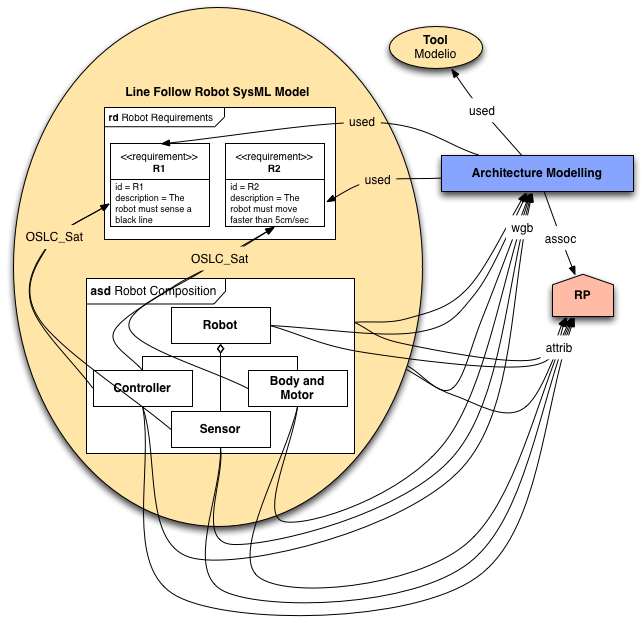
\includegraphics[width=0.8\textwidth]{figures/Traceability/step02}
\caption{Traceability links captured during the production of an ASD for a line following robot.}\label{fig:traceability:step02}
\end{figure}

%\draftnote{CJG: As the user(s) use the tools, they each record the their atomic actions, forming the traceability graph}

A development project will likely consist of many instances of the activities identified in the ontology being performed and together they form a traceability graph.  Figure~\ref{fig:traceability:abstractTraceFlow} shows a simplified view of a traceability graph with some steps removed for brevity.  At the top of the graph we see the architecture modelling step described previously, that produces an architecture model.  From the architecture, model description files are exported to start the production of the simulation models.  In turn the simulation models are exported as FMUs and the FMUs are used to produce simulation results.  Key to the traceability graph then are the 'used' and 'wgb' connections that can be used by a query to determine from where each entity was generated.  By following these links back from any entity to the individual blocks within the architecture model, it is possible to determine which requirement(s) each should satisfy.  Finally when simulation results are output, these may be linked back to the relevant requirements, stating whether a requirement was verified or violated by that result.

%\draftnote{CJG: Give abstract view of a resulting trace}


\begin{figure}[htbp]
	\centering
	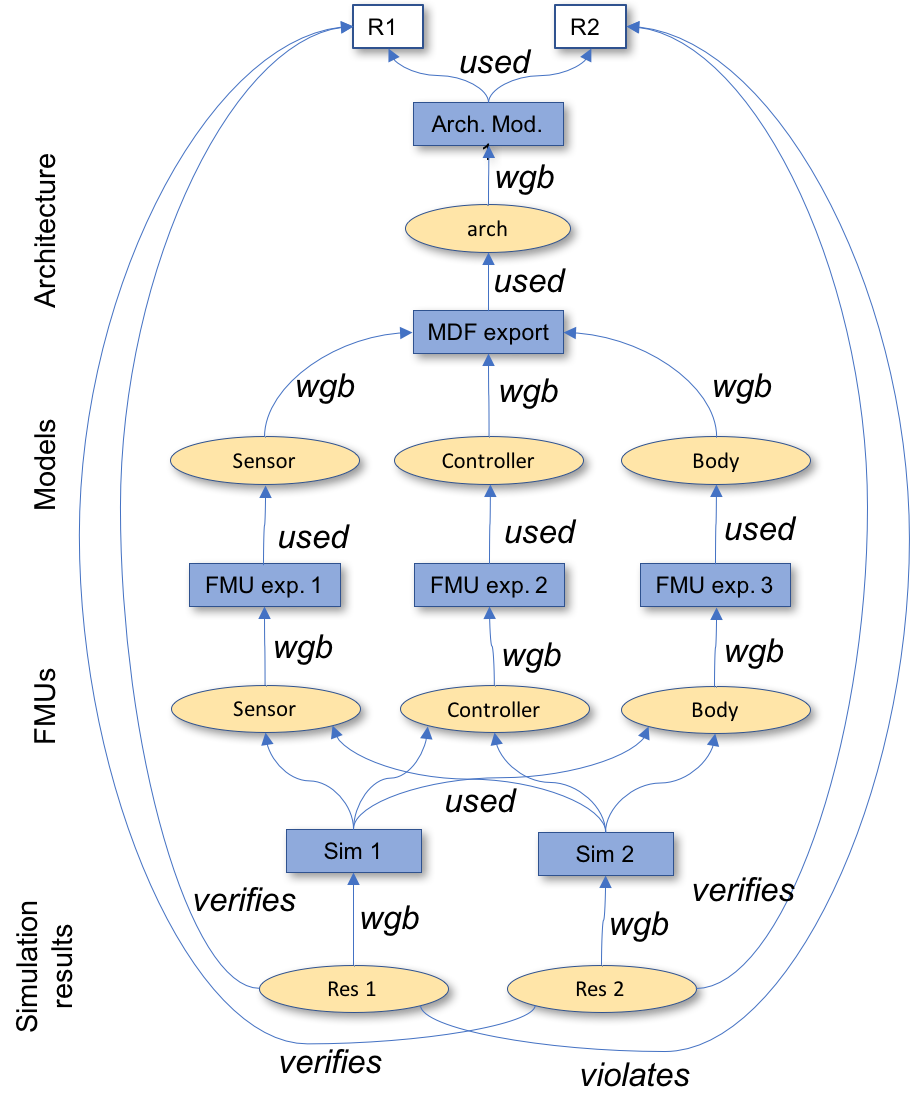
\includegraphics[width=0.7\textwidth]{figures/Traceability/abstractTraceFlow}
\caption{Traceability links captured during the production of an ASD for a line following robot.}\label{fig:traceability:abstractTraceFlow}
\end{figure}


%\draftnote{CJG: A paragraph outlining the entities, activities and agents}

The traceability ontology captures the significant activities and entities that form the INTO-CPS workflow.  For example a development project might see the following activities recorded in the traceability graph:  \emph{Requirements Management}, \emph{Architecture Modelling}, \emph{Architecture Configuration Creation} \emph{Model Description Export}, \emph{Simulation Modelling}, \emph{FMU Export}, \emph{Configuration Creation}, \emph{Simulation Configuration Creation} and then \emph{Simulation}.  These activities are connected in the workflow by the entities they create and use, so the example would see the traceability graph containing records of: \emph{Archtecture Structure Diagram}, \emph{Architecture SubSystem}, \emph{Architecture Connection Diagram}, \emph{Model Description File}, \emph{Simulation Model}, \emph{FMU}, \emph{Multi-model Configuration}, \emph{Simulation Configuration} and \emph{Simulation Result}.  Alongside these will be records of the agent(s), who are both associated with activities and have entities attributed to them.


Once a graph has been built, queries can be executed over the graph to perform both forwards and backwards traceability. Below are some types of queries that can be executed over the graphs. Examples include: forward traceability (from requirements to entities); backwards traceability (from FMU to requirements); finding sources and sinks for a simulation; assessing coverage such as finding requirements without positive simulation results; and evaluating user impact, such as finding all artefacts influenced by a given user.

\subsubsection{Requirements Engineering}
\label{sec:method:reqeng}

Requirements placed on a CPS may, for example, impose restrictions, define system capabilities or identify qualities of a system. The requirements should indicate some value or use for the different stakeholders of a CPS. Traceability needs requirements to be defined early in a development process, and these must be recorded in Modelio for the machine-assisted traceability information to be recorded accurately. It is therefore appropriate to consider requirements processes for such developments at this stage.

In the INTO-CPS Methods guidelines~\cite{INTOCPSD3.3b}, we describe one possible approach to RE for CPS, adapting an approach already piloted on tsystems-of-systems (SoSs). Note however that this approach is not mandatory, and in general RE processes and tools vary widely across organisations and domains. For this reason, tool support for traceability in INTO-CPS begins once requirements have been defined and can be added to Modelio. The approach was adapted from standard systems engineering, and tailored for SoSs--- enabling the identification and reasoning about requirements across constituent systems of an SoS and understanding multi-stakeholder contexts. We suggest it might be useful to organisations trying to approach RE for CPS.

In the approach, we propose a collection of views that could be represented as diagrams in SysML\footnote{Note that this approach is is not specifically supported as a Modelio plug-in, but other equivalent diagrams could be used.}, or could equally be represented in other tools where these are already used (e.g. Excel). Examples of views include:

\begin{description}
\item[Source Element View (SEV)] which defines a collection of source materials from which requirements are derived. This could be represented as a SysML block definition diagram ior an Excel table or Word document (with each source having a unique identifier), or by simply referring to source documents using OSLC traces.

\item[Requirement Description View (RDV)] which is used to define the requirements of a system and forms the core of the requirement definition. This can be done in a SysML requirements diagram or in tabulated form, such as through the use of Excel. In addition, specifying requirements in  Doors would support this view.

\item[Context Definition View (CDV)] The CDV is a useful view for CPS engineering in order to explicitly identify interested stakeholders and points of context in the system development, including customers, suppliers and system engineers themselves. In SoS-ACRE, they are defined using SysML block definition diagrams, and could also be represented using an Excel table or Word document (with each context having a unique identifier). This diagram type could be useful when identifying the divide in CT/DE and cyber-physical elements of a system.

\item[Requirement Context View (RCV)] In SoS-ACRE, a RCV is defined for each constituent system context identified in CDVs. This is appropriate when there is a set of diverse system owners, which is typical for SoSs and increasingly CPSs. A \textbf{Context Interaction View (CIV)} is then defined to understand the overlap of contexts and any common/conflicted views on requirements. In a CPS, however, there may not be such a clear delineation between the owners of constituent  system components. However, if we consider the different domains (e.g. CT/DE or cyber/physical divides) as different contexts, then this approach would be useful. In SoS-ACRE, RCVs and CIVs are both defined with SysML use case diagrams. Excel could be used if unique identifiers are defined for contexts and requirements as described earlier.

\item[Validation View (VV)] VVs, defined as SysML sequence diagrams in SoS-ACRE, describe validation scenarios for a SoS to ensure each constituent system context understands the correct role of the requirements in the full SoS. This is not an obvious fit in CPS engineering, and therefore not necessarily required.

\end{description}

The full RE process is described in greater detail in \cite{INTOCPSD3.3a} as a disciplined approach involving identifying and recording source elements (in an SEV), system-level functional and non-functional requirements (using RDVs), an initial system structure (in an INTO-CPS ASD, which identified cyber and physical elements), and relevant contexts in CDVs. Requirements may then be traced using INTO-CPS tool chain models and results.

\subsubsection{SysML and Multi-modelling}
\label{sec:method:sysml}

Standard SysML can be used as part of a development process to build a model of a system and link elements to requirements. The INTO-CPS tool chain also provides an extended SysML profile that help users to \emph{configure multi-models for co-simulation} and \emph{configure design space exploration (DSE) analysis}~\cite{INTOCPSD2.1a,INTOCPSD2.2a,INTOCPSD2.3a,INTOCPSD41c,INTOCPSD4.2c,INTOCPSD4.3c}.
The multi-modelling SysML profile defines two diagrams for configuring a co-simulation. The INTO-CPS Application can run a co-simulation based on a configuration file which describes the FMUs, their parameters and connections between them. There are two types diagram, the \emph{Architectural Structure Diagram (ASD)} describing the static structure of FMUs, and the \emph{Connections Diagram (CD)} describing their instantiation and connections. These are shown in Figure~\ref{fig:sysml:intocps}.

\begin{figure}[h!]
\centering
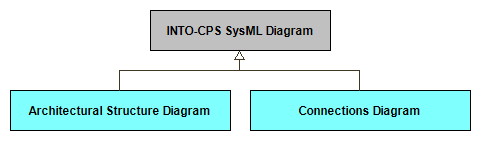
\includegraphics[scale=0.6]{figures/Architecting/ArchitecturalViews}
\caption{Diagrams in the multi-modelling SysML profile}
\label{fig:sysml:intocps}
\end{figure}

The design space exploration (DSE) SysML profile is an addition to the multi-modelling SysML profile described above. As with single co-simulation, the INTO-CPS Application can run a DSE based on a configuration file. Alternatively, a configuration can be generated by Modelio, from a set of diagrams defined in the profile. There are five diagram types (see Figure~\ref{fig:sysml:dse} which are used to define the objectives for a DSE and their instantiations, define the parameters that will be changed on each co-simulation in a DSE and their instantiations, and the objectives to be used for ranking competing designs.

\paragraph{Holistic and Design Architectural Modelling}
\label{sec:sysml:holistic}

A system architecture defines the major components of a system, and identifies their relationships, behaviour and interactions. A model of the architecture is potentially partial (representing some or all of the system) and abstract, limited to those elements pertinent to the modelling goal. In CPS engineering, this goal may include understanding the system in terms of the application domain (a \emph{holistic} model), or capturing the system components in a way that targets multi-modelling (a \emph{design} model).

The diagrams in the two profiles described above divide architectural models into subsystems composed of cyber or physical components. Defining an architecture this way may not be the best approach when designing a system ab initio, with systems comprising entities across different domains requiring diverse domain expertise. The Methods Guidelines~\cite{INTOCPSD3.3a} discusses and exemplifies both holistic and design architectural modelling approaches, and provides some commentary and guidance on how to model in a way which is natural for domain experts, and how to move from holistic to design models when multi-modelling.


\paragraph{Representing Non-Design Elements in SysML}
\label{sec:sysml:non-design}

Using the INTO-CPS tool chain, we generate co-simulation configurations using an architectural model defined with the INTO-SysML profile. This model defines the structure of a system in terms of the composition of its components and their connections. There are however circumstances where elements in the multi-model are not part of the design of the final system, for example where an FMU is used purely for visualisation. This FMU must be connected to the system components, however is not itself a system component. This is also true when considering the environment of the system. The Methods Guidelines~\cite{INTOCPSD3.3a} presents an example of the use of these extensions.

\subsubsection{A `DE-first' Approach to Developing Multi-models}

After carrying out requirements engineering (RE), and design architectural modelling in SysML the engineering team should have  Architecture Structure Diagrams (ASDs) defining the composition of components to be realised as FMUs in cyber or physical formalisms, along with model descriptions exported for each component, and some Connections Diagrams (CDs) that will be used ot configure a multi-model. The next step is to generate a multi-model configuration in the INTO-CPS Application and populate it with FMUs, then run a first co-simulation. This however requires the source models for each FMU to be ready. If they already exist this is easy, however they may not exist if this is a new design. In order to generate these models, the model descriptions for each component can be passed to relevant engineering teams to build the models, then FMUs can be passed back to be integrated.

It can be useful however to create and test simple, abstract FMUs first (or in parallel), then replace these with higher-fidelity FMUs as the models become available. This allows the composition of the multi-model to be checked early, and these simple FMUs can be reused for regression testing. This approach also mitigates the problem of modelling teams working at different rates.

Where these simple FMUs are built within the DE formalism (such as VDM), this is called a \emph{DE-first} approach. This approach is particularly appropriate where complex DE control behaviours ---such as supervisory control or modal behaviours--- are identified as a priority or where the experience of the modelling team is primarily in the DE domain~\cite{Fitzgerald&14c}. Guidance on how to produce DE approximations for use in multi-modelling, and in particular approximations of CT behaviour, can be found in material describing the Crescendo baseline technology~\cite{Fitzgerald&13a}, which is also available via the Crescendo website\footnote{See \url{http://crescendotool.org/documentation/}}.

In INTO-CPS, given an architectural structure diagram, connections diagram and model descriptions for each component, the suggested approach is to begin by building a single VDM-RT project in Overture with: a class for each component representing an FMU' a `system class' that instantiates port and FMU objects based on the connections diagram, and a `world' class that starts the thread of each FMU object. FMUs can be exported and co-simulated within the INTO-CPS tool. These FMUs can then be replaced as higher-fidelity versions become available, however they can be retained and used for regression and integration testing by using different multi-model configurations for each combination.

\subsubsection{Modelling Networks with VDM in Multi-models}
\label{sec:method:networks}
When modelling and designing distributed controllers, it is necessary to model communications between controllers as well. While controller FMUs can be connected directly to each other through for co-simulation, this quickly becomes unwieldy due to the number of connections increasing exponentially. We suggest employing an `ether' pattern in which a representation of an abstract communications medium is introduced~\cite{Fitzgerald&14c}. In the INTO-CPS setting, the ether is an FMU that is connected to each controller that handles message-passing between them. This reduces the number of connections needed, particularly for large numbers of controllers such as swarms. In the Methods Guidelines~\cite{INTOCPSD3.3a}, we describe how to pass messages between VDM FMUs using string types, how the ether class works, some of the consequences of using the ether pattern, and finally some extensions for providing quality of service (QoS) guarantees. 


\subsubsection{Design Space Exploration}
\label{sec:method:dse}

In this section, we outline guidelines for DSE over multi-models of CPSs. These are intended to (a) support decision management by helping engineers to articulate clearly the parameters, objectives and metrics of a DSE analysis; and (b) enable the tuning of DSE methods for given domains and systems of interest. Engineers need to be able to model at an early stage of design how DSE experiments relate to the model architecture, and where possible trace from requirements to the experiments. The Methods Guidelines describe the first step towards this vision: a SysML profile for modelling DSE experiments. As mentioned in Section~\ref{sec:method:dse}, the profile comprises five diagrams for defining \emph{parameters}, \emph{objectives} and \emph{rankings}.

The Methods Guidelines~\cite{INTOCPSD3.3a} present an illustrative example of the use of the DSE-SysML profile -- from requirements engineering through defining parameters and objectives in the DSE-SysML profile to the final DSE configuration files. 

DSE is performed in the DSE tool (see the INTO-CPS User Manual~\cite{INTOCPSD4.3a}) by processing the DSE configuration using scripts that contain the required algorithms.  The main scripts contain the search algorithm that determines which parameters to use in each simulation, the simplest of these is the exhaustive algorithm that methodically runs through all combinations of parameters and runs a simulation of each.  The log files produced by each simulation are then processed by other scripts to obtain the objective values defined in the previous section.  Finally, the objective values are used by a ranking script to place all the simulation results into a partial order according to the defined ranking.  The ranking information is used to produce tabular and graphical results that may be used to support decisions regarding design choices and directions.

Figure~\ref{fig:dse-results} shows an example of the DSE results from a line follower robot where the lap time and mean cross track error were the objectives to optimise.  These results contain two representations of the data, a graph plotting the objective values for each design, with the Pareto front of optimal trade-offs between the key objectives highlighted, here in blue. The second part of the results presents the data is tables, indexed by the ranking position of each result.  This permits the user to determine the precise values for both the measured objectives and also the design parameters used to obtain that result.

\begin{figure}[h!]
	\centering
	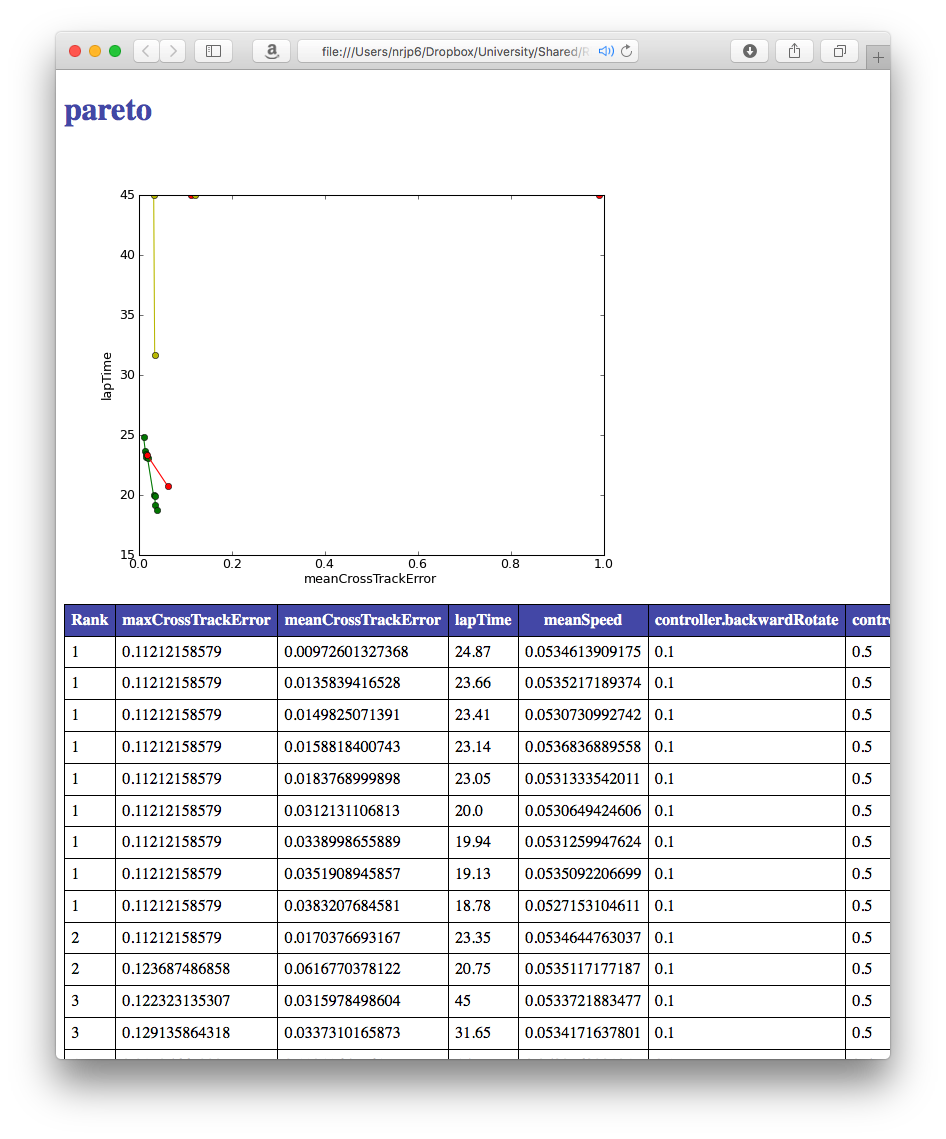
\includegraphics[width=0.9\textwidth]{figures/dse_results}
	\caption{DSE results}
	\label{fig:dse-results}
\end{figure}

\paragraph{An Approach to Effective DSE}
\label{sec:dse-algorithms}

Given a ``designed'' design space using the method detailed above, we use the INTO-CPS Tool Chain to simulate each design alternative. Whilst this approach is acceptable on small-scale studies, it quickly becomes infeasible as the design space grows. Inspired by processes found in nature, genetic algorithms ``breed'' new generations of optimal CPS designs from the previous generation's best candidates. This mimics the concept of survival of the fittest in Darwinian evolution.
Figure~\ref{fig:ga_dse_process} outlines the structure of a genetic algorithm used for DSE.  Several activities are reused from exhaustive DSE: simulation; evaluation of objectives; rank simulated designs; and generate results. The remaining activities are specific to the genetic approach and are detailed in the Methods Guidelines~\cite{INTOCPSD3.3a}.

\begin{figure}[h!]
	\centering
	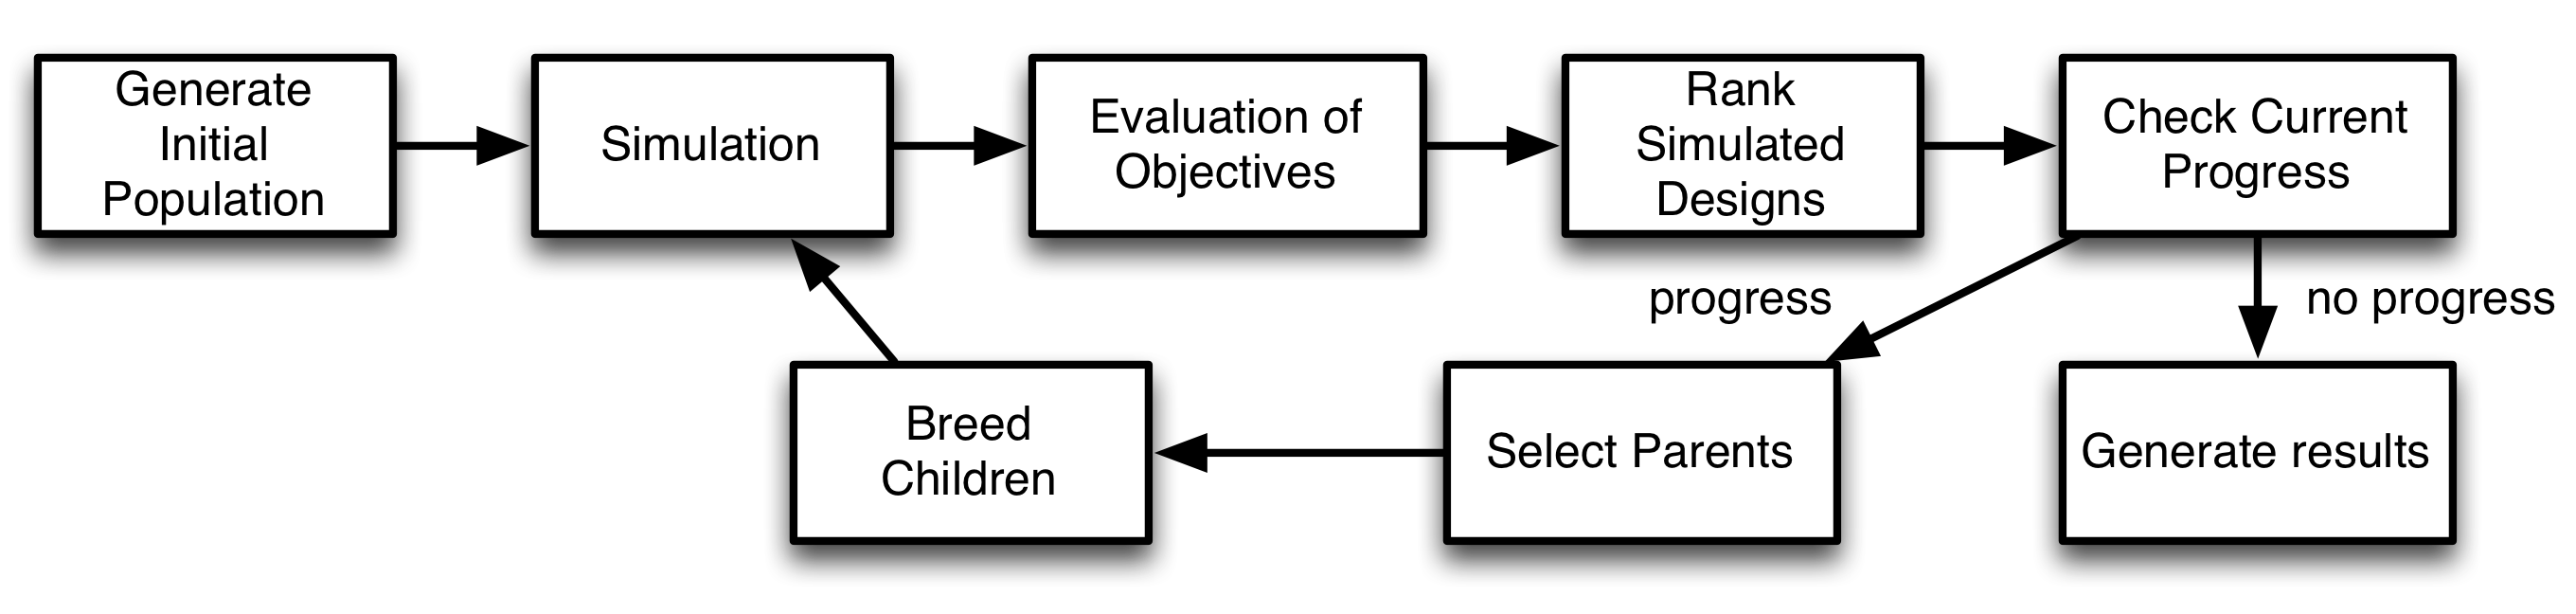
\includegraphics[width=0.9\textwidth]{figures/ga_process}
	\caption{High-level process for DSE Genetic Algorithm}
	\label{fig:ga_dse_process}
\end{figure}


An alternative to the genetic search, which is automated, is to use repeated exhaustive searches to home in on better regions of the design space.  In this approach the user would plan to perform multiple DSE experiments, each using some portion of their total simulation budget.  The first DSE experiment is used to cover the whole range of the design space, but not including all values for each parameter.   In this way the first DSE is used to locate regions of interest within the design space.  The regions of interest are areas of the design space that produced the better designs according to the ranking results, with the bounds of the 'area' defined by the parameter values that produced good results. The user then divides up their remaining simulation budget between the one or more areas of interest and perform further DSE on those areas.  

\clearpage
%!TEX root = ../INTO-CPS-Manifesto.tex

\section{The INTO-CPS Tool Chain}\label{sec:toolchain}

\fbox{Christian K\"{o}nig with support from Etienne Brosse}

\fbox{make sure that this section fits to the other sections, incl. references}

\fbox{indicate maturity of the different tool features, in particular wrt. the new ones}

This section discusses the interconnectivity of the different tools, and how the tools fit into the workflows and tasks that are covered by INTO-CPS. In particular, this section focuses on the features that were added during the INTO-CPS project, and in the framework of the INTO-CPS association. This section does \textit{not} describe all the tools in detail (here, the reader is referred to the different manuals, and to the User Manual (ref to the INTO-CPS tool manual).

An overview of the different tools that form the tool-chain of the INTO-CPS association, is given in Figure \ref{fig:tool-chain}.

[text on the overall tool-chain, refer to workflows, probably from previous section]

\begin{figure}[!ht]
	\centering
		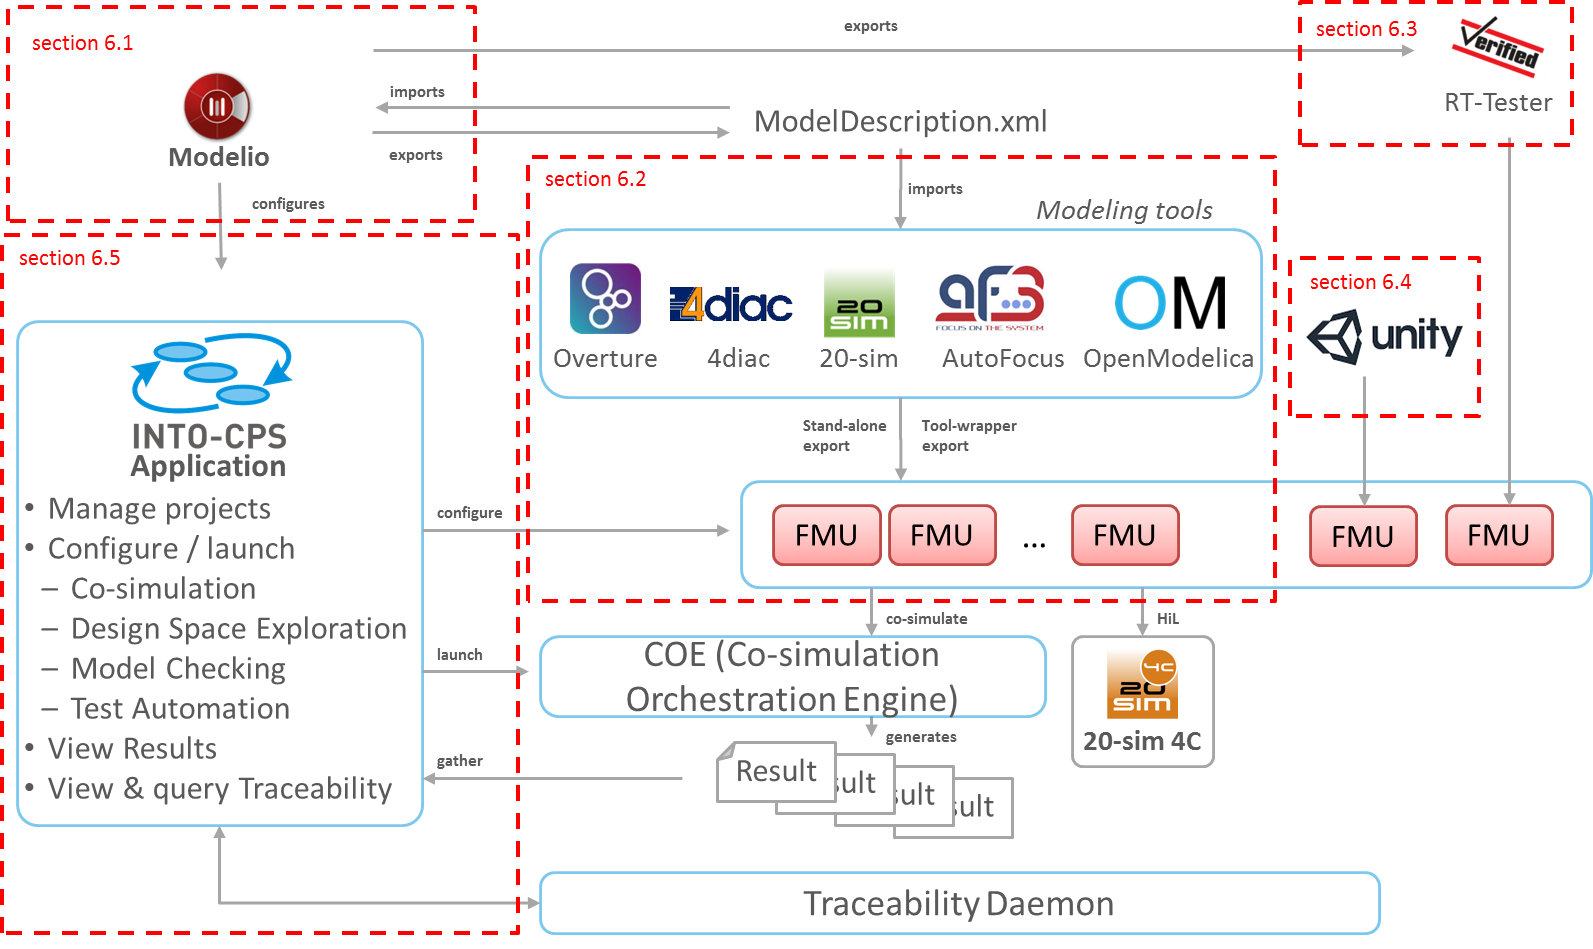
\includegraphics[width=0.9 \textwidth]{./figures/toolchain_association}
	\caption{Overview of the different tools and their arrangement in a tool-chain.}
	\label{fig:tool-chain}
\end{figure}
%[Figure of the overall tool-chain]

\subsection{Modelio}
\label{sec:modelio}
Modelio is an open-source modelling environment for various formalisms with many interfaces to import and export models. In the context of INTO-CPS, the support for SysML modelling is of primary importance, while Modelio can be extended with a range of modules to enable more modelling languages. In the terminology of the methods guidelines (e.g. \cite{INTOCPSD3.3a}), Modelio is a tool for the \textit{architectural modelling} and for \textit{requirements management}.

During the INTO-CPS project, a SysML profile was created, which is currently available as a module for Modelio 3.4 and 3.6 (see \url{http://forge.modelio.org/projects/intocps}). This INTO-CPS SysML profile extends Modelio with several functionalities that described in detail elsewhere (refs). Here, only those parts of the INTO-CPS SysML profile are discussed that add features for interconnectivity in the tool-chain.

To support the FMI multi-modelling approach, \texttt{ModelDescription.xml} files can now be imported into, and exported from a SysML Architectural Modelling diagram. Importing ModelDescription.xml files creates a SysML block with the corresponding flow ports and attributes, exporting them allows import in other modelling tools, such as those described below.

The Connections Diagram describes the signal flow between the different SysML blocks, which can each correspond to one FMU. Using the new INTO-CPS SysML profile, the Connections Diagram can be exported to an intermediary JSON format, which can then be imported by the INTO-CPS Application, to create a new Multi-Model.

%The INTO-CPS SysML Profile\\
%Import of ModelDescription.xml \\
%Export of ModelDescription.xml files (for modeling tools)\\
%Export of Connections Diagram (for the Application)\\

Diagrams for handling of Design Space Exploration (DSE) were created for Modelio, also included in the INTO-CPS SysML profile. These diagrams allow connection of parameters with signals, definition of objectives for a DSE, connection of signals with objectives, and ranking of results. Using these diagrams, a complete DSE configuration can be exported from Modelio.

Behavioural models that are designed in Modelio as state machines can be exported as \texttt{.xmi} files, so that they can be imported to the RT Tester tools

%DSE modeling configuration\\
Requirements management\\
Traceability\\

\subsection{Modelling tools}

At the core of the tool-chain are several modelling tools that describe a system or a sub-system in a specific formalism, and perform calculations to understand the dynamic behaviour of the (sub-)system. While the formalisms or application areas can be vastly different, the modelling tools share some common features, which are summarized in this section. 

\paragraph{20-sim} is a commercial tool for modelling and simluation of mechatronic systems. Together with the related software, 20-sim 4C, Hardware-in-the-Loop simulations can be performed. \url{http://www.20sim.com/}

\paragraph{OpenModelica} is an open-source environment which is based on the Modelica language. It features numerous free libraries to easily model systems from different domains. \url{https://openmodelica.org/}

\paragraph{Overture} is an open-source tool that supports the modelling method \textit{The Vienna Development Method (VDM)}, which is a formal method to describe computing systems. \url{http://overturetool.org/}

\paragraph{4Diac} is an open-source tool for distributed process measurement and control systems based on the IEC 61499 standard. \url{https://www.eclipse.org/4diac/}

\paragraph{AutoFocus3} is an open-source model based tool to develop embedded software systems. \url{https://af3.fortiss.org/}

\paragraph{Cossim}

\paragraph{ABS}

Most modelling tools support the same functions in the context of INTO-CPS. A \texttt{ModelDescription.xml} file (e.g.\ one that is automatically created from Modelio, see previous section) can be imported to create a skeleton model with the input and output signals and exposed parameters. After the actual modelling work is done, the model can be exported as Functional Mock-up Unit (FMU), in accordance with the FMI 2.0 for Co-Simulation standard. This FMU can either contain all the necessary models and solvers, so that is a self-contained model (also called stand alone), or it contains libraries which call a simulation tool to execute the simulation. The latter case is called a tool wrapper FMU. Furthermore, the different steps of importing, saving and exporting generate traces which are sent to the traceability engine of the INTO-CPS Application. The following table summarizes the status of the different tools at the time of writing of this document.

\begin{table*}[ht]
	\centering
		\begin{tabular}{l|p{2.5cm}|p{2.5cm}|p{2.5cm}|p{2.5cm}}
			Tool & MD.xml import & FMU import & FMU export (stand alone) & FMU export (tool wrapper) & Traceability\\
			\hline
			20-sim & yes & yes & no & yes & yes\\
			OpenModelica & yes & yes & yes & no & yes\\
			Overture & yes & yes & yes & yes & yes\\
			4diac & no & no & under development & no & no \\
			AutoFocus 3 & no & under development & no & no & no\\
			Cossim & N.A. & N.A. & N.A. & N.A. & N.A. \\
			ABS & no & no & no & planned & no \\
		\end{tabular}
	\caption{Functionalities of the modelling tools}
	\label{tab:FunctionalitiesOfTheModelingTools}
\end{table*}

\subsection{RT Tester}

In the framework of INTO-CPS, the RT Tester tool suite (see \url{https://www.verified.de/products/rt-tester/}) is extended with mainly two objectives: Integration of Test-Automation and of Model Checking in the INTO-CPS tool-chain. Both functions are integrated into the INTO-CPS application, and both support traceability.

\subsubsection{Test Automation}

Test Automation within INTO-CPS uses the RT Tester tools to generate, perform and analyze tests, based on Co-simulation of a system. The Test Automation functionalities are integrated into the INTO-CPS Application. The behavioural model can be generated in Modelio, and exported as \texttt{.xmi} file, which in turn can be read by RT Tester. After the test is created in RT Tester, the test procedure can be cast into an FMU file. Together with a Co-Simulation scenario, and using the COE, the test procedure is used to run a test project. More information on Test Automation in INTO-CPS can be found in \cite{INTOCPSD5.3b}.

\subsubsection{Model Checking}

Model checking in INTO-CPS is used to verify system properties of multi-models, consisting of continuous-time (CT) and discrete-event (DE) models. Similar to the Test Automation features, Model Checking is based on the RT Tester tool suite. From a tool-chain perspective, Model Checking is integrated in the INTO-CPS Application, which allows the complete configuration, execution and analysis of a Model Checking experiment. More information on Model Checking in INTO-CPS can be found in \cite{INTOCPSD5.3c}.


\subsection{3D animation}

The 3D animation FMU allows visualisation of the simulation. It is based on the Unity engine (see \url{https://unity3d.com}), and extends it by exporting the scenario and the 3D rendering as a FMU \cite{Foldager&17}. The Modelio SysML profile (see Section \ref{sec:modelio}) takes the visualisation FMU into account. The 3D animation FMU also supports Virtual Reality (VR) headsets. It has been used in multiple case studies of INTO-CPS [ref].

\subsection{The INTO-CPS Application}

The INTO-CPS Application is the central tool to integrate the different tools and artefacts, to configure and run simulations, manage results, and more. It allows configuration and execution of DSE scenarios (which can be imported from Modelio), and is a front-end for Model-checking and Test automation, by using the RT Tester tool. Furthermore, traceability data can be viewed in the Application, either in an expert view, using the Neo4J visualisation\footnote{\url{https://neo4j.com/}}, or by pre-configured queries.

%Integration of the different artifacts\\ 
%configuration and execution of Co-Simulation\\
%Front-end for Test-automation and model checking\\
%Viewer for traceability\\

\clearpage
% !TeX root = ../INTO-CPS-Manifesto.tex



\section{The INTO-CPS Industrial Case Studies}\label{sec:casestudies}

\fbox{Stylianos Basagiannis}

\subsection{Integrated product-production co-simulation for cyber-physical production system (iPP4CPPS) } 

The case study involved the virtual design and validation of a CPS-based manufacturing system for assembling USB sticks, inspired from Continental's real manufacturing and testing processes in a production line. It is a representative example of distributed heterogeneous systems in which products, manufacturing resources, orders and infrastructure are all cyber-physical. In this setting, several features (such as asynchronous communication, messages flow, autonomy, self-adaptation, etc.) could be investigated at design time, for example using a collaborative modelling approach. Consequently, the case study offered a balance between being sufficiently simple to be easily followed as a production line example, including generating a tangible output, and at the same time being sufficiently general to allow the study of the co-simulation complexity. Furthermore, by choosing a USB stick, the example opened the (unexplored) possibility of extending the purpose of the study to interactions between generated hardware and generated software solutions in the production line.

Obviously, this small experiment, in terms of scale and time, could not give a full and clear assessment of benefits for developing an integrated product-production co-simulation for CPS-based industrial control. Nevertheless, there were some recognisable benefits compared to the current state of technology:

\begin{itemize}
\item the possibility to simulate, test and validate from a holistic perspective and with an increased level of accuracy an entire production system that needs cross-functional expertise; The initial development of a homogeneous co-simulation in VDM for the iPP4CPPS prototype was particularly useful in driving cooperation and making clear the assumptions of the distributed teams involved in modelling the specific components. This phase proved to be the most difficult and time-consuming in building the co-simulation, requiring a very intensive communication for a shared understating of the requirements. Once the VDM co-simulation was running, the independent developments of units could be integrated, validated and deployed in any order.
\item to a certain extent, the ability to handle unpredictable integration requirements. The employment of co-simulations when designing an automated production system avoided the build-up inertia of subsequent design constraints, facilitating the low and late commitment for these decisions, i.e.\ the specific microcontrollers or PLCs, the layout of the plant, the number of memory boxes from the warehouse etc. For example, the possibility to generate code - from all the simulation tools used in this experiment (i.e.\ 4DIAC, 20-Sim, Overture) -- for an extended set of computational devices was a clear advantage in respect to late commitment for the computational system used in the production system. 
\end{itemize}

The methodology adopted in the IPP4CPPS project to develop the co-simulation closely followed the classical stages of agent-oriented or component-based software engineering methodologies. Following the mechanical model derived from the requirements, the high-level abstraction for the behaviour of each simulation was implemented and the interactions among the components could be analysed. It included distinct simulations for each component type (Table 1): production (i.e.\ warehouse station, robot, transporting wagons, and testing station), orders (i.e.\ placed via mobile devices), and factory infrastructure (i.e.\ part tracker). 

The co-simulation model had been initially implemented in VDM and validated on the INTO-CPS tools chain. The main goal of this implementation was manifold: a) to validate the interaction protocols among the composite simulations; b) to have an early working co-simulation where the specific simulations may be gradually added, tested and validated; c) to allow for a more independent development among the dispersed teams involved in modeling the specific simulations, while at the same time keeping the co-simulation functional at all times; and d) to cover the left-over parts of the co-simulation whose modelling was not needed in detail for the validation of the interaction protocol (e.g. test station) or for which there is was FMI-compliant tool (i.e.\ factory infrastructure).   

\begin{table*}[ht]
	\centering
		\begin{tabular}{|p{2.4cm}|p{1.8cm}|p{3.2cm}|p{4cm}|}\hline
			\textbf{Component type} & \textbf{Unit} & \textbf{Technology} & \textbf{Deployment}\\
			\hline\hline
			Orders & HMI & 4DIAC + MQTT \textit{or} Overture (VDM) & smartphones and tablets \\ \hline
			Infrastructure & Part Tracker & Overture (VDM) & NVIDIA Tegra Jetson\\ \hline
			Production & Warehouse + Robotic Arm & 20-sim & Raspberry Pi with UniPi Expansion Board + Stäubli robot\\ \hline
			Production & Wagons & 4DIAC & Raspberry Pi controlling DC motors, position sensors and anti-collision ultrasonic sensors \\ \hline
			Production & Test Station & 4DIAC & Cognex Vision Insight 1100 camera connected to Raspberry Pi for actuators control\\ \hline
			General & Unity & 20-sim animation & PC\\\hline
		\end{tabular}
	\caption{Technologies used for different system components}
	\label{tab:iPP4CPPS_technologies}
\end{table*}

The detailed model of each simulation covered a continuous-time model realised in 20-Sim for the warehouse and robotic arm, a discrete-time model in 4DIAC for the transportation system and test station, and a discrete-time model in Overture for the infrastructure. All units modelled and tested by the heterogeneous co-simulation were then deployed in a demo stand for fine tuning under real-life conditions (Table \ref{tab:iPP4CPPS_technologies}). This phase presumed the extension of code generation capabilities of the simulation tools, such as: 20-sim 4C has been extended with MQTT, Modbus, I2C color sensor, I2C multiplexer and UniPi board for the Raspberry Pi; Overture for employing MQTT as communication protocol on a Raspberry Pi 3; and 4DIAC for accelerometers control. 

\begin{figure}[!ht]
	\centering
		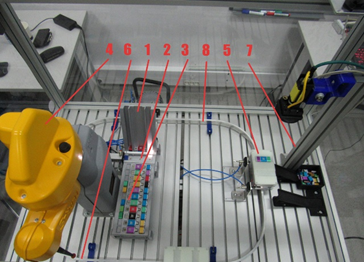
\includegraphics[width=0.9 \textwidth]{./figures/demo_stand}
	\caption{Demo stand for deployment of the co-simulated units, containing: 1) the warehouse stacks; 2) the assembly box at the base of the warehouse stacks; 3) the memory boxes of the warehouse unit; 4) the robotic arm for moving parts around the warehouse; 5) wagons on different locations of the track; 6) the loading station; 7) the test station; 8) the circular track for the wagons..}
	\label{fig:demo_stand}
\end{figure}

The experiment assessed the benefits and the maturity level of model-driven engineering technologies for future adoption into CPS-based production systems. It covered the entire engineering life-cycle (i.e. from requirements to deployment into a real infrastructure) and contributed to several advancements of engineering methods and tools. The experiment delivered an effective proof-of-concept for model-driven engineering of CPS-based production system as a feasible and promising approach to (re)engineer the factory of the future with the employed technologies (i.e.\ INTO-CPS, Overture, 20-Sim and 4DIAC). Nevertheless, the experiment also identified a number of issues that may have further impact over the adoption of model-driven engineering technologies into real settings: the FMI-compatibility of the simulation tools used in industry; the hardware/software-in-the-loop simulations still display complex synchronisation problems for dissimilar time-scales; the extended set of low-level devices (i.e.\ sensors, industrial communication standards etc.) that are used in today and future industry require special standardisation effort to enhance the deployment capabilities of the simulation tools\footnote{More information can be found at \url{http://centers.ulbsibiu.ro/incon/index.php/ipp4cpps/} and \url{http://www.cpse-labs.eu/experiment.php?id=c3_uk_gs_ipp4cpps}.}

\subsection{Use of the INTO-CPS Technology at MAN Diesel \& Turbo}

As reported in \cite{Pedersen&17}, at \ac{mdt} the conventional approach for
developing two-stroke combustion engines with a distributed embedded control
system is being challenged. In particular, for diesel engines pollution is a
key element that it is desirable to reduce from a competitive perspective. New
emission legislation focuses on the reduction of especially NO$_x$ emission.
Widely known emission reduction technologies for reducing NO$_x$ are selective
catalytic reduction and \ac{egr}, both being developed at \ac{mdt}
\cite{Pedersen&17}.

These systems require advanced algorithms to control the complexity of the
physical dynamics of large engines. \ac{mdt} is divided into different
departments with different responsibilities in the same way as many other large
organisations. In the control department at \ac{mdt}, control algorithms are
created directly in the target software framework with the possibility of
performing \ac{sil} simulation during development.  Models of the physical
behaviour are created in other departments of \ac{mdt} using the tools most
suitable for the specific constituent system.  

For the control system development, the physical dynamics models are
implemented in an internally developed tool for \ac{ct} simulation called the
\ac{mdse} which is part of the software framework. The primary focus in
\ac{mdse} is \ac{sil}/\ac{hil}, and the physics models implemented here are
often an abstraction of high-fidelity models. Historically it has been
challenging inside \ac{mdt} to enable heterogeneous collaborations between the
different teams producing models in different departments. As a result
different models are typically fragmented and solely used within one department
for the dedicated purpose each of the models serve. Thus, efforts that goes
across these individual insights are only found at the test on the real
platform.


%% Change this paragraph
At \ac{mdt} the models used in the control department are based on a software
framework and \ac{mdse} is implemented in C++ and run on a 32-bit Linux
platform while the physical modelling tools often require Windows. During the
INTO-CPS project it was illustrated how a transition from the current
simulation process at \ac{mdt} to one using co-simulation utilising the
\ac{fmi} standard can be performed by using the \ac{coe} from the \ac{intocps}
project. The aim with the approach suggested was to reduce redundancy in the
development process and reuse and combine models from different
departments \cite{Pedersen&17}. One of the main challenges for such a transition
is to enable co-simulation across different hardware architectures and \ac{os}
platforms due to constraints from software frameworks, physical simulation
tools and version compatibility, and INTO-CPS Technology was key in overcoming
it.


\clearpage
% !TeX root = ../INTO-CPS-Manifesto.tex

\section{Related Work}\label{sec:related}

Extensive work has been done to identify the main concepts and essential challenges in co-simulation.
In this section, we review some of these works.

\cite{Trcka2007} reviews principles and implementation strategies of co-simulation applied to an HVAC system.
It provides multiple experiments showing how the stability and accuracy of the co-simulation is affected by the choice of those strategies.

The work in \cite{Hafner2017} exposes the disparity in terminology related to co-simulation (e.g., the term ``co-simulation'' is understood as ``cooperative simulation'', or ``coupled system simulation''), provides an in-depth discussion of the multiple concepts, and proposes a way to classify and structure co-simulation methods.
The authors propose the distinction by:
\begin{compactdesc}
\item[state of development:] the motivation being the use of co-simulation (e.g., optimise the simulation of a single model by partitioning, or couple the behavior of wildly different subsystems);
\item[application field:] see, e.g., the application fields described in \cite{Gomes2017};
\item[model description:]  the kind of models being combined (e.g., Ordinary Differential Equations (ODEs), Differential-Algebraic Equations (DAEs), discrete event systems);
\item[numerical approach:] the kind of coupling algorithms employed; and
\item[interfaces:]  the nature of the physical interfaces between the systems being coupled.
\end{compactdesc}

Recognizing that co-simulation is not a new concept and that it has been applied in wildly different fields, \cite{Gomes2018} reviewed co-simulation approaches, research challenges, and research opportunities. 
They apply feature oriented domain analysis \cite{Kang1990} to help map the field. 
The main result is a feature model that classifies the requirements of co-simulation frameworks and the participating simulators. 
They conclude that the main research needs are: finding generic approaches for modular, stable, valid, and accurate coupling of simulation units; and finding standard interfaces for hybrid co-simulation. 

With a focus on power systems, but still covering the fundamental concepts, \cite{Palensky2017} highlights the value of co-simulation for the analysis of large scale power systems. 
In a tutorial fashion, it goes over the main concepts and challenges, providing a great introduction for new researchers in the field.

Recognising the research in co-simulation should be driven by both industry and academia, \cite{Schweiger2018a} reports on an empirical survey, given to both practitioners and academics.
The preliminary results \claudio{(An extended version is being published at the American Modelica Conference)} corroborate the challenges pointed out in the surveys we referenced here.
Additionally, it becomes clear that co-simulation is being used without in-depth knowledge of the subject, which may lead to the improper use of the technique, as well as highlighting the need to develop more usable tools.

Finally, \cite{Gomes2018b} discusses the past and future of co-simulation, providing an historical overview of the topic, as well as possible research directions.

\claudio{Should we survey also co-simulation frameworks, or are the above surveys on the topic enough?
I guess that if someone wants to learn about co-simulation, the surveys are a better way to start\ldots}

\clearpage
% !TeX encoding = UTF-8
% !TeX spellcheck = en_GB
% !TeX root = ../INTO-CPS-Manifesto.tex
%
%
%
\section{Future Directions}\label{sec:future}

%\fbox{Peter Gorm Larsen}

It is envisaged that the INTO-CPS technology will be further extended as the FMI standard evolves and in particular in future research projects. 
Thus, the future directions here will depend both on the members of the INTO-CPS Association as well as which externally funded research projects that will be successful in achieving funding. 

In the subsections below candidate future directions are proposed.

\subsection{Adapting FMUs Easily to Ones Needs}

In the context of continuous system co-simulation, it is well known that there is no one-size-fits-all co-simulation approach. 
Different kinds of systems are best co-simulation different ways (cite survey).
At the same time, different domains have specialised numerical solvers, which means we cannot ignore the solvers in the FMUs.
A future research direction is to understand how to reconcile such contradicting requirements.
A possible way is to allow the user to preserve the exported FMUs, but change the way these interact with the environment, by wrapping an FMU around them \cite{Gomes&18a}.
This way does not solve all challenges in this regard, and the approach lacks validation from multiple domains. It is envisaged that this kind of Domain Specific Languages (DSLs) will be developed to make it easier to make semantic adaptations of FMUs.

%\claudio{Maybe providing``connector'' FMUs for the most common connections in different domains. For example, if I'm building a co-simulation of an hydraulic system, I may want to connect a large pipe to a small pipe.}

\subsection{Enlarging the tools and standards supported by the INTO-CPS Tool Suite}

The INTO-CPS tool suite is on purpose open to any tool that live up to the requirements in the FMI version 2.0 standard for co-simulation. As indicated in Section~\ref{sec:toolchain} a possible entry point to the co-simulation setup is a special SysML profile supporting CPS models. Right now this is discussed in OMG as a potential new standard in a SysML setting and this is only supported by the Modelio tool (supporting export of both model descriptions as well as configurations of co-simulation). It would be great to see this special profile by other SysML tools as well. In addition, one can imagine that alternative tool supporting AADL \cite{AADL04} or Capella \cite{Roques17}.

There are also a lot of other standards for co-simulations \cite{Gomes&18} and it is possible to imagine that bridges from the INTO-CPS tool chain will be made to a number of these. Here the most obvious candidate is High Level Architecture (HLA) \cite{IEEE1516}. Initial work has been carried out in other research groups for such a combination \cite{Neema&14,Awais&17} but we imagine that more work is needed here to get this combination working smoothly.

%\claudio{Can you elaborate on this? What does supporting more tools mean? Also, which standards are we talking about? HLA?}

\subsection{Use in a Cloud-based Eco-system/Marketplace}

The INTO-CPS Application is made using Electron so it is using web technology but still requires local installation on the local computers. It is possible to imagine that it will be possible to move this to become a cloud application where it will no longer be necessary to install it locally. The DSE feature is already available in a cloud context as explained above. In a very long context it can also be imagined that the different modelling and simulation tools at some stage will become available on-line and possibly in a cloud context.

In addition to the tools becoming available in a cloud context one can imagine that it some point in the future will be possible to share constituent models in a cloud context. Such models could then either be available in a source form or a generated form in the form of an FMU. Optimally these could include both free as well as commercial models in a marketplace setting. We believe that this could enable a shortage of time required to develop multi-models for CPSs.

\subsection{Use in a Digital Twin setting}

In order to increase the value of multi-models one can imagine making use of them in a deployed setting, i.e., after the CPS has been deployed if data from it can be fed back to a cloud where a co-simulation can be used to predict how alternative interventions can be made and what the consequences of these will be \cite{Gamble&18}. This is known as a \emph{digital twin} but there are naturally a number of research challenges in connection with something like this since you need to determine how to set up such a co-simulation as well as what the consequences will be of the frequency of the data arriving in pseudo-real-time. For some types of application this could work, whereas for others the predictions would be far from representing reality. Research is needed to determine when this would work.

%\claudio{I can't understand what exactly this entails.
%Maybe it is best to describe the case studies that we want to support?
%To me, supporting digital twin entails at least enhancing the COE for real-time co-simulation (to use in a diagnosing use case)}

\subsection{Increased Support for Dynamic Evolution Scenarios}

In a System of System setting it is regular that the composition of constituent systems involved in a scenario change dynamically over time. In an FMI setting this is currently not possible since it is necessary to have a static composition of the FMUs used in a co-simulation. In order to be able to support dynamic evolution in a co-simulation scenario it is desirable to conduct research exploring to what extend this could be a possibility.

%\claudio{Not clear what dynamic evolution means\ldots Is this supporting incremental development (having multiple refinements of the same component?) Isn't this related to traceability?}

\subsection{Incorporation of Computational Fluid Dynamics Co-simulations}

To accurately model flow of material (typically liquid or gasses) Computational Fluid Dynamics (CFD) models are typically used. These are typically represented at a very detailed level, and as a consequence CFD simulations can be really slow. In addition, in case CFD simulations fail the error control is not properly aligned with the orchestration enabled in a FMI based setting. In order to properly support CFD elements in an INTO-CPS setting research is needed to determine how this can be carried out efficiently in a semantically sound manner. Here it is imagined that a part of this will be approximating the CFDs with Reduced Order Models (ROMs) \cite{Carlberg&13}.

%\claudio{Might be easier to describe the use cases in concrete. For example, I think the into-cps can already support CFD co-simulations (you just need the FMUs to do that\ldots). What is does not support is error control techniques, that can kick in when CFD co-simulations are run.}

\subsection{Increased support for Human Interaction}

Human-in-the-Loop where people can give input to co-simulations while they are running is certainly relevant. This have actually been carried out both using the PVSio technology on the line following robot example \cite{Palmieri&17}. In addition, human intervention has been used in a part of co-simulations in the IPP4CPPS project (see Section~\ref{sec:IPP4CPPS}). However, we imagine that substantial more automation and assistance can be made for this kind of human interaction. One can also imagine that debugging features such as pausing, inspecting values and possibly injecting faults could be included in the Co-simulation Orchestration Engine.

%\claudio{Can you provide example advancements to support this? Example, real-time co-simulation seems an easy one. Maybe the ability to pause, inspect, and debug co-simulations?
%Maybe fault injection?}

\subsection{Increased support for Network Considerations}

FMI is not by itself good at modelling the communication layers between different constituent systems. In the INTO-CPS project it was attempted to model this as an FMU ether where messages can be lost. However, it would be ideal to be able to appropriate model each FMU being at a particular address (e.g., a URL or an IP address) and then have a library of alternative connections between such addresses, where one could experiment with non-ideal behaviour (e.g., delays and loosing messages). Such non-ideal behaviour may actually influence the way the real system behaves and thus it makes a lot of sense that it also would be possible to incorporate such aspects at a modelling level so it could be analysed either in plain co-simulations or with DSEs.

%\claudio{What does this entail? Adding delays to the signals? Adding noise? Is this related to semantic adaptation or fault injection?}

\subsection{Intelligence, Adaptivity and Autonomy}

CPSs also ideally are smart in the sense that they process intelligent behaviour. In order to introduce autonomy it can be ideal to introduce Machine Learning (ML) in different fashions in order to lear how to best behave. ML can be used in different ways here:

\begin{itemize}
\item Based on time series data for an individual physical component one can imagine that ML can be used to automatically derive an approximation FMU corresponding to that physical component
\item In a digital twin setting one can imagine that ML can be used to learn to what extend the real system behave as predicted by the co-models. Based on this different actions could be taken automatically or manually if human intervention is desirable.
\item FMUs themselves could contain ML elements for example in order to have adaptive control that will be valuable and express intelligent behaviour.
\end{itemize}

%\claudio{We need to make this more concrete. Do we mean the co-simulation of adaptive systems?
%Are we looking at variable structure systems? Or the development of a COE that is adaptive (nice challenge, to ensure stability with adaptive master algorithms)?
%Also, another possible direction is to support certification processes by, e.g., having built in mechanisms to calculate the errors being made (during or after the co-simulation is run).
%This is interesting because the user just has to provide the bounds he can tolerace, and the co-simulation will be run as many times as required, so that these tolerances are met.
%Another possible direction is to support hybrid co-simulation (even when there is no possibility of rolling back from the FMUs).
%}

\subsection{Tradeoff in Abstraction between Speed and Accuracy}

Many models can be expressed at different levels of abstraction. There is a natural tradeoff between speed and accuracy of a co-simulation. 
An interesting direction could for example be to support DSE's, while using multiple abstraction models.
For example, higher abstraction models might be used to optimise the design globally, while lower abstraction models validate the candidate found, and further optimise each of them to find the best one. In particular for FMUs that are very slow in simulating (e.g., CFD models) it may make a lot of sense to use more abstract models (at least initially) in order to be able to obtain results within a reasonable amount of time. For CFD models it is for example possible to produce Reduced Order Models (ROMs) and these can be automatically derived from more detailed models. Thus, it can be valuable to make it easy for users to select what level of abstraction to use in a co-simulation for each of the constituent models.


\clearpage
%
%
%
%
%%%% Bibliography %%%%
\bibliographystyle{alpha}
\bibliography{bibliography,intocps,intocpsdev,foundations}
\label{ch:bib} %label to refer to
%
%
%
\clearpage
%
%
%
\appendix
\section{List of Acronyms}\label{appendix:acronyms}
\begin{longtable}{ll}
20-sim	& Software package for modelling and simulation of dynamic sys\allowbreak\@tems\\
%ACA     &Automatic Co-model Analysis\\
%ACC	&American Control Conference\\
%ARM	&Advanced Risc Machines\\
%AFD     &Anticipatory Failure Determination\\
%AHU     & Air Handling Unit\\
API & Application Programming Interface \\
%ARTEMIS	&Advanced Research and Technology for Embedded Intelligence and Systems\\
%ASIC	&Application-Specific Integrated Circuit\\
AST     & Abstract Syntax Tree\\
%ATC & Automatic Train Control\\
%ATE     & Atego\\
AU      & Aarhus University\\
%BAN     &Body Area Network\\
BCS & Basic Control States \\
%BMBF    &German Ministry of Research and Education\\
%BMC     &Bounded Model Checker\\
%BMS     &Building Management System\\
%BRIC    &Brazil, Russia, India and China\\
%BODERC	&Beyond the Ordinary: Design of Embedded Real-time Control\\
%BSCW	&Be Smart, Cooperate Worldwide\\
%CA	&Consortium Agreement\\
%CAD	& Computer Aided Design\\
%CAST    &Certification Authorities Software Team\\
%CACSD	&Computer-Aided Control System Design\\
%CHAMP   &The CPS Heterogeneous and Agile Modelling Platform\\
%CDE     &Collaborative Development Environment\\
CFD & Computational Fluid Dynamics\\
%CHP     &Combined Heat Power\\
%CIT     &Cork Institute of Technology\\
%CLE     & ClearSy\\
CLP	&Controllab Products B.V. \\
%CML     &COMPASS Modelling Language\\
%CMM	&Capability Maturity Model\\
%CMMI	&Capability Maturity Model Integrated\\
%CO	&Confidential\\
COE & Co-simulation Orchestration Engine \\
%COMPASS &Comprehensive Modelling for Advanced Systems of Systems\\
%CoNES   & Complex Networked Embedded Systems\\
CORBA & Common Object Request Broker Architecture \\
%CPLab   &Cyber-Physical systems Lab\\
CPS     & Cyber-Physical Systems\\
%CPU	&Central Processing Unit\\
%CSER	&Conference on System Engineering Research\\
%CSP	&Communication Sequential Processes\\
CT	&Continuous-Time\\
%CTC++	&Communicating Threads library for C++\\
%CTQ	&Criticals to Quality\\
%DAL     &Development Assurance Level\\
%DARPA   &Defense Advanced Research Projects Agency, USA\\
%DATE	&Design, Automation and Test in Europe\\
%DCSC	&Dependable Computing Systems Centre\\
DE      &Discrete Event\\
%DESCA   &DEvelopment of a Simplified Consortium Agreement for FP7\\
DESTECS	&Design Support and Tooling for Embedded Control Software\\
%DG      &Distributed Generators\\
%GNSS    &Global Navigation Satellite System\\
%GPS     &Global Positioning System\\
DSE	&Design Space Exploration\\
DSL & Domain Specific Language \\
%DSO     &Distributed System Operators\\
%DSN	&Dependable Systems and Networks\\
%DSP	&Digital Signal Processor\\
%EASST	&European Association of Software Science and Technology\\
%EC	&European Commission\\
%EDA	&Electronic Design Automation\\
%EMSOFT	&Embedded Systems Software\\
%ENG     & Department of Engineering\\
%ERP     &Enterprise Resource Planning\\
%ESA	&European Space Agency\\
%EV  &Electrical Vehicle\\
%FDL	&Forum on Design Languages\\
%FDR     &Failures Divergences Refinement\\
%FM	&Formal Methods\\
%FMEA    &Failure Mode and Effects Analysis\\
FMI     &Functional Mockup Interface\\
FMI-Co  &Functional Mockup Interface -- for Co-simulation\\
FMI-ME  &Functional Mockup Interface -- Model Exchange\\
%FMTC    &Functional Mockup Trust Centre\\
FMU     &Functional Mockup Unit\\
%FPGA	&Field-Programmable Gate Array\\
%FT	&Fault Tolerance\\
%FTA     &Fault Tree Analysis\\
%GA      & General Assembly\\
%GNU	&GNU's Not Unix\\
%GSN     &Goal Structuring Notation\\
%HEV     &Hybrid Electric Vehicle\\
HiL	&Hardware-in-the-Loop\\
HLA & High-Level Architecture \\
HMI     &Human Machine Interface\\
%HVAC    &Heating, Ventilation, and Air Conditioning\\
HW      &Hardware\\
ICT	&Information Communication Technology\\
IDE	&Integrated Design Environment\\
%IFG	&Industry Follow Group\\
%IFM	&Integrated Formal Methods\\
%INCOSE	&International Council on Systems Engineering\\
%IPA     &Information-technology Promotion Agency, Japan\\
%IPP     &Innovation Pilot Program\\
%IPR     & Intellectual Property Right\\
%ISO	&International Organisation of Standards\\
%ISOLA	&International Symposium on Leveraging Applications of Formal Methods\\
%ITEA 	&Information Technology for European Advancement\\
%KK      &Kongskilde Industries\\
%KPI     &Key Performance Indicator\\
%LE	&Large Enterprise\\
%LNCS	&Lecture Notes in Computer Science\\
LTL & Linear Temporal Logic \\
%LV      &Low Voltage\\
M\&S    &Modelling and Simulation\\
MARTE & Modeling and Analysis of Real-Time and Embedded Systems\\
MBD     &Model-based Design\\
MBT & Model-based Testing\\
MC/DC   &Modified Decision/Condition Coverage\\
MDE & Model Driven Engineering \\
%MG      &Micro Generators\\
%MGT	&Management of the consortium\\
MiL 	&Model-in-the-Loop\\
MIWG & Model Interchange Working Group\\
%MV      &Medium Voltage\\
%NSF     &National Science Foundation, USA\\
%OA      &Open Access\\
%OEM	&Original Equipment Manufacturer\\
OMG     &Object Management Group\\
%OLMECO	&Open Library for MEchatronic COmponents\\
OS	&Operating System\\
%PC      &Project Coordinator\\
PID     &Proportional Integral Derivative \\
%PLC & Programmable logic controller\\
%PM	&Person Months	\\
%PMO     & Project Management Office\\
%PB      &Project Board\\
%PP	&Restricted to other Programme Participants\\
%PPE     &Project Planning \& Execution\\
%PPP     &Product Passport Process\\
%PROSPER	&Proof and Specification Assisted Design Environments\\
PROV-N  &The Provenance Notation\\
%PV      &Photovoltaic\\
%PU	&Public	\\
%QA	&Quality Assurance\\
%QMP	&Quality Management Plan\\
%RATP    &R\'{e}gie Autonome des Transports Parisiens (a public transport operator)\\
%ReSIST	&Resilience for Survivability in IST\\
%RLC     &Remote Load Control\\
%RODIN	&Rigorous Open Development Environment for Complex Systems\\
RPC     &Remote Procedure Call\\
%RSU     &Research Support Unit\\
%RTD	&Research and Technological Development\\
%RTK     &Real-Time Kinematics\\
RTT & Real-Time Tester\\
%RTP     & Reference Tool Platform\\
%RUP	&Rational Unified Process\\
%S\&T    &Science \&\ Technology\\
%SACM    &Structured Assurance Case Metamodel\\
%SAL     &Symbolic Analysis Laboratory\\
%SCADA   &Supervisory Control And Data Acquisition\\
%SE      &Software Engineering\\
%SEFM	&Software Engineering Formal Methods\\
%SIL	& Safety Integrity Level\\
SiL	& Software-in-the Loop\\
%SME	&Small Medium Enterprise\\
SMT & Satisfiability Modulo Theories \\
%SoS     &System of Systems\\
%SOS     &Structural Operational Semantics‎\\
%SotA    &State-of-the-Art\\
%SPI     &System Properties Intervals \\
%SRA	&Strategic Research Agenda\\
ST      &Softeam\\
SUT     &System Under Test\\
SVN	&Subversion\\
%SW      &Software\\
SysML	&Systems Modelling Language\\
TA      &Test Automation\\
%TBD	&To Be Determined\\
%TDD     &Test Driven Development\\
TE & Test Environment\\
%TIA	&Telecommunications Industry Association\\
TR & TRansitions \\
TRL     &Technology Readiness Level\\
%TRNSYS  &TRaNsient SYstems Simulation \\
TWT & TWT GmbH Science \& Innovation\\
UML	&Unified Modelling Language\\
UNEW	&University of Newcastle upon Tyne\\
%UO      &Utility Operators\\
%UTC     &United Technologies Corporation\\
UTP     &Unifying Theories of Programming\\
UTRC    & United Technologies Research Center\\
UY      & University of York\\
VDM     &Vienna Development Method\\
%VICE	&VDM++ In Constrained Environments\\
VSI     & Verified Systems International\\
%V\&V    &Validation \&\ Verification\\
%WAM     &Weighted Additive Method\\
WP	&Work Package\\
%WPL	&Work Package Leader\\
%WT	&Wind Turbines\\
XML	&Extensible Markup Language\\
\end{longtable}

\clearpage
\section{Underlying Principles}
\label{appendix:principles}
The INTO-CPS tool chain facilitates the design and validation of CPSs through its implementation of results from a number of underlying principles.
%
These principles are co-simulation, design space exploration, model-based test automation and code generation.
%
This appendix provides an introduction to these concepts.
%
%
%
\subsection{Co-simulation}
Co-simulation refers to the simultaneous simulation of individual models which together make up a larger system of interest, for the purpose of obtaining a simulation of the larger system.
%
A co-simulation is performed by a co-simulation orchestration engine.
%
This engine is responsible for initializing the individual simulations as needed;  for selecting correct time step sizes such that each constituent model can be simulated successfully for that duration, thus preventing time drift between the constituent simulations;  for asking each individual simulation to perform a simulation step;  and for synchronizing information between models as needed after each step.
%
The result of one such round of simulations is a single simulation step for the complete multi-model of the system of interest.

As an example, consider a very abstract model of a nuclear power plant.
%
This consists of a nuclear reactor core, a controller for the reactor, a water and steam distribution system, a steam-driven turbine and a standard electrical generator.
%
All these individual components can be modelled separately and simulated, but when composed into a model of a nuclear power plant, the outputs of some become the inputs of others.
%
In a co-simulation, outputs are matched to inputs and each component is simulated one step at a time in such a way that when each model has performed its simulation step, the overall result is a simulation step of the complete power plant model.
%
Once the correct information is exchanged between the constituent models, the process repeats.
%
%
%
\subsection{Design Space Exploration}
During the process of developing a CPS, either starting from a completely blank canvas or constructing a new system from models of existing components, the architects will encounter many design decisions that shape the final product.
%
The activity of investigating and gathering data about the merits of the different choices available is termed Design Space Exploration.
%
Some of the choices the designer will face could be described as being the selection of parameters for specific components of the design, such as the exact position of a sensor, the diameter of wheels or the parameters affecting a control algorithm.
%
Such parameters are variable to some degree and the selection of their value will affect the values of objectives by which a design will be measured.
%
In these cases it is desirable to explore the different values each parameter may take and also different combinations of these parameter values if there are more than one parameter, to find a set of designs that best meets its objectives.
%
However, since the size of the design space is the product of the number of parameters and the number of values each may adopt, it is often impractical to consider performing simulations of all parameter combinations or to manually assess each design.

The purpose of an automated DSE tool is to help manage the exploration of the design space, and it separates this problem into three distinct parts:  the search algorithm, obtaining objective values and ranking the designs according to those objectives.
%
The simplest of all search algorithms is the exhaustive search, and this algorithm will methodically move through each design, performing a simulation using each and every one.
%
This is termed an open loop method, as the simulation results are not considered by the algorithm at all.
%
Other algorithms, such as a genetic search, where an initial set of randomly generated individuals are bred to produce increasingly good results, are closed loop methods.
%
This means that the choice of next design to be simulated is driven by the results of previous simulations.

Once a simulation has been performed, there are two steps required to close the loop.
%
The first is to analyze the raw results output by the simulation to determine the value for each of the objectives by which the simulations are to be judged.
%
Such objective values could simply be the maximum power consumed by a component or the total distance traveled by an object, but they could also be more complex measures, such as the proportion of time a device was operating in the correct mode given some conditions.
%
As well as numerical objectives, there can also be constraints on the system that are either passed or failed.
%
Such constraints could be numeric, such as the maximum power that a substation must never exceed, or they could be based on temporal logic to check that undesirable events do not occur, such as all the lights at a road junction not being green at the same time.
%

The final step in a closed loop is to rank the designs according to how well each performs.
%
The ranking may be trivial, such as in a search for a design that minimizes the total amount of energy used, or it may be more complex if there are multiple objectives to optimize and trade off.
%Unless there is a trivial goal for the system, such as simply minimising energy used, then there is a need for the final part of closed loop, which is to rank designs according to their objective values and their ability to meet the constraints set out for them.
%
Such ranking functions can take the form of an equation that returns a score for each design, where the designs with the highest/lowest scores are considered the best.
%
Alternatively, if the relationship between the desired objectives is not well understood, then a Pareto approach can be taken to ranking, where designs are allocated to ranks of designs that are indistinguishable from each other, in that each represents an optimum, but there exist different tradeoffs between the objective values.  
%
%
%
\subsection{Model-Based Test Automation}
The core fragment of test automation activities is a model of the desired system behaviour, which can be expressed in SysML.
%
This test model induces a transition relation, which describes a collection of execution paths through the system, where a path is considered a
sequence of timed data vectors (containing internal data, inputs and outputs).
%
The purpose of a test automation tool is to extract a subset of these paths from the test model and turn these paths into test
cases, respectively test procedures.
%
The test procedures then compare the behaviour of the actual system-under-test to the path, and produce warnings once discrepancies are observed.
%
%
%
%\subsection{Model Checking}
%Naturally, model checking applied to a co-simulation environment is not dissimilar to model checking of distributed systems, which are formed from independent components. 
%%
%The purpose is to verify properties of the entire system, consisting of numerous components that run in parallel.
%%
%There is one important dissimilarity, however.  In INTO-CPS, the system structure consists of heterogeneous models, and these different components may be specified using different formalisms, or the entire system may even employ simulations, auto-generated code and real hardware controllers.
%%
%This observation leads to the need for a uniform representation of models -- no matter how they are implemented -- that can be used for model checking purposes, and naturally, for a precise notion of abstraction.
%
%To apply model checking to an INTO-CPS multi-model, there is one more challenge when integrating components of different kinds.
%%
%Some of the components may, for example, depend on the calculation of differential equations, for which model checking is intractable except for the smallest examples.
%%
%The drive to analyze and verify real-world systems thus forces us to represent complex components by their abstract counterparts, which are again expressed as timed state charts.
%%
%That is, all models need to be represented as discrete event models.
%
%The key idea in abstraction is to represent a concrete model $\mathcal{M}$ by a more abstract counterpart $\alpha(\mathcal{M})$ by application of an abstraction function $\alpha$.
%%
%In essence, $\alpha$ must be designed so that $\alpha(\mathcal{M})$ describes all behaviours originally presented in $\mathcal{M}$, and possibly additional ones.
%%
%Thus, abstraction preserves safety properties: If a safety property holds for the abstract model
%$\alpha(\mathcal{M})$, then the property also holds for the concrete model $\mathcal{M}$.
%%
%However, since $\alpha$ may introduce additional behaviours, checking $\alpha(\mathcal{M})$ may lead to false positive warnings: a property
%violation may be reported for $\alpha(\mathcal{M})$, but the violated behaviour is not part of the concrete model $\mathcal{M}$. Details on how $\alpha$ can be implemented are described in~\cite{INTOCPSD51c}.
%
%Apart from the need for abstraction, the topology of the model connection is more involved for co-simulation as implemented in INTO-CPS.
%%
%The overall system design does not consist of a single system-under-test, but rather a collection of systems whose inputs and outputs are connected using a graph-like structure.
%
%With respect to the turn indication example from Section~\ref{appendix:rtt-model-checking} (Figure~\ref{figure:vsi-simple}), the same behaviour may be implemented by two independent controllers, one for each side.
%%
%Then, the overall system topology is connected as given in Fig.~\ref{figure:vsi-more-complex}.
%%
%By using this kind of modelling, where different system models are all included as timed state charts, it is possible to specify LTL formulae as before.
%%
%This form of modelling connections between system components, however, is an integral part of the INTO-CPS project.
%%
%Model checking in the context of INTO-CPS thus smoothly integrates with the overall INTO-CPS approach.
%%
%%
%%
%\begin{figure}
%\centerline{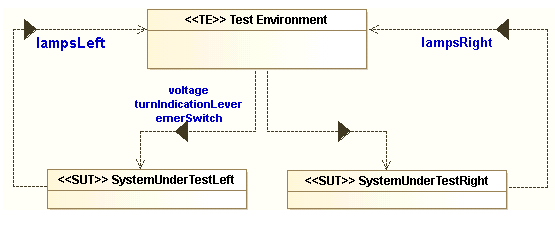
\includegraphics[width=\textwidth]{figures/VSI-modelio-more-complex.png}}
%\caption{Extension of the system topology sketched in
%  Fig.~\ref{figure:vsi-simple}.}
%\label{figure:vsi-more-complex}
%\end{figure}
%
%
%
\subsection{Code Generation}
Code generation refers to the translation of a modelling language to a common programming language.
%
Code generation is commonly employed in control engineering, where a controller is modelled and validated using a tool such as 20-sim, and finally translated into source code to be compiled for some embedded execution platform, which is its final destination.

The relationship that must be maintained between the source model and translated program must be one of refinement, in the sense that the translated program must not do anything that is not captured by the original model.
%
This must be considered when translating models written in high-level specification languages, such as VDM.
%
The purpose of such languages is to allow the specification of several equivalent implementations.
%
When a model written in such a language is translated to code, one such implementation is essentially chosen.
%
In the process, any non-determinism in the specification, the specification technique that allows a choice of implementations, must be resolved.
%
Usually this choice is made very simple by restricting the modelling language to an executable subset, such that no such non-determinism is allowed in the model.
%
This restricts the choice of implementations to very few, often one, which is the one into which the model is translated via code generation.

\clearpage
%!TEX root = ../INTO-CPS-Manifesto.tex
\section{Background on the Individual Tools}
\label{appendix:tools}
This appendix provides background information on each of the independent tools of the INTO-CPS tool chain.
%
%
%
\subsection{Modelio}\label{app:modelio}
Modelio is a comprehensive MDE \cite{Favre05} workbench tool which supports the UML2.x standard.
%
Modelio adds modern Eclipse-based graphical environment to the solid modelling and generation know-how obtained with the earlier Softeam MDE workbench, Objecteering, which has been on the market since 1991.
%
Modelio provides a central repository for the local model, which allows various languages (UML profiles) to be combined in the same model, abstraction layers to be managed and traceability between different model elements to be established.
%
Modelio makes use of extension modules, enabling the customisation of this MDE environment for different purposes and stakeholders.
%
The XMI module allows models to be exchanged between different UML modelling tools.
%
Modelio supports the most popular XMI UML2 flavors, namely EMF UML2 and OMG UML 2.3.
%
Modelio is one of the leaders in the OMG Model Interchange Working Group (MIWG), due to continuous work on XMI exchange improvements.

Among the extension modules, some are dedicated to IT system architects.
%
For system engineering, SysML or MARTE modules can be used.
%
They provide dedicated modelling support for dealing with general, software and hardware aspects of embedded or cyber physical systems.
%
In addition, several utility modules are available, such as the Document Publisher which provides comprehensive support for the generation of different types of document.

Modelio is highly extendable and can be used as a platform for building new MDE features.
%
The tool enables users to build UML2 Profiles, and to combine them with a rich graphical interface for dedicated diagrams, model element property editors and action command controls.
%
Users can use several extension mechanisms: light Python scripts or a rich Java API, both of which provide access to Modelio‘s  model repository and graphical interface.
%
%
%
\subsection{Overture}\label{app:overture}
The Overture platform \cite{Larsen&10a} is an Eclipse-based integrated development environment (IDE) for the development and validation of system specifications in three dialects of the specification language of the Vienna Development Method.
%
Overture is distributed with a suite of examples and step-by-step tutorials which demonstrate the features of the three dialects.
%
A user manual for the platform itself is also provided \cite{Larsen&13a}, which is accessible through Overture's help system.
%
Although certain features of Overture are relevant only to the development of software systems, VDM itself can be used for the specification and validation of any system with distinct states, known as \emph{discrete-event systems}, such as physical plants, protocols, controllers (both mechanical and software) \emph{etc}.\@, and Overture can be used to aid in validation activities in each case.

Overture supports the following activities:
%
%
%
\begin{itemize}
%
\item  The definition and elaboration of syntactically correct specifications in any of the three dialects, via automatic syntax and type validation.
%
\item  The inspection and assay of automatically generated proof obligations which ensure correctness in those aspects of specification validation which can not be automated.
%
\item  Direct interaction with a specification via an execution engine which can be used on those elements of the specification written in an executable subset of the language.
%
\item  Automated testing of specifications via a custom test suite definition language and execution engine.
%
\item  Visualization of test coverage information gathered from automated testing.
%
\item  Visualization of timing behaviours for specifications incorporating timing information.
%
\item  Translation to/from UML system representations.
%
\item  For specifications written in the special executable subset of the language, obtaining Java implementations of the specified system automatically.
%
\end{itemize}
%
%
%

For more information and tutorials, please refer to the documentation distributed with Overture.

The following is a brief introduction to the features of the three dialects of the VDM specification language.
%
\paragraph{VDM-SL}
This is the foundation of the other two dialects.
%
It supports the development of monolithic state-based specifications with state transition operations.
%
Central to a VDM-SL specification is a definition of the state of the system under development.
%
The meaning of the system and how it operates is conveyed by means of changes to the state.
%
The nature of the changes is captured by state-modifying operations.
%
These may make use of auxiliary functions which do not modify state.
%
The language has the usual provisions for arithmetic, new dependent types, invariants, pre-\@ and post-conditions \emph{etc}.
%
Examples can be found in the VDM-SL tutorials distributed with Overture.
%
\paragraph{VDM++}
The VDM++ dialect supports a specification style inspired by object-oriented programming.
%
In this specification paradigm, a system is understood as being composed of entities which encapsulate both state and behaviour, and which interact with each other.
%
Entities are defined via templates known as \emph{classes}.
%
A complete system is defined by specifying \emph{instances} of the various classes.
%
The instances are independent of each other, and they may or may not interact with other instances.
%
As in object-oriented programming, the ability of one component to act directly on any other is specified in the corresponding class as a state element.
%
Interaction is naturally carried out via precisely defined interfaces.
%
Usually a single class is defined which represents the entire system, and it has one instance, but this is only a convention.
%
This class may have additional state elements of its own.
%
Whereas a system in VDM-SL has a central state which is modified throughout the lifetime of the system, the state of a VDM++ system is distributed among all of its components.
%
Examples can be found in the VDM++ tutorials distributed with Overture.
%
\paragraph{VDM-RT}
VDM-RT is a small extension to VDM++ which adds two primary features:
%
%
%
\begin{itemize}
%
\item  The ability to define how the specified system is envisioned to be allocated on a distributed execution platform, together with the communication topology.
%
\item  The ability to specify the timing behaviours of individual components, as well as whether certain behaviours are meant to be cyclical.
%
\end{itemize}
%
Finer details can be specified, such as execution synchronisation and mutual exclusion on shared resources.
%
A VDM-RT specification has the same structure as a VDM++ specification, only the conventional system class of VDM++ is mandatory in VDM-RT.
%
Examples can be found in the VDM-RT tutorials distributed with Overture.
%
%
%
\subsection{20-sim}\label{app:20sim}
{20-sim} \cite{20sim,Broenink97} is a commercial modelling and simulation software package for mechatronic systems.
%
With {20-sim}, models can be created graphically, similar to drawing an engineering scheme.
%
With these models, the behaviour of dynamic systems can be analysed and control systems can be designed.
%
{20-sim} models can be exported as C-code to be run on hardware for rapid prototyping and HiL-simulation.
%
{20-sim} includes tools that allow an engineer to create models quickly and intuitively.
%
Models can be created using equations, block diagrams, physical components and bond graphs \cite{Karnopp&68}.
%
Various tools give support during the model building and simulation.
%
Other toolboxes help to analyse models, build control systems and improve system performance.
%
%
%
\begin{figure}[hpt!]
	\centerline{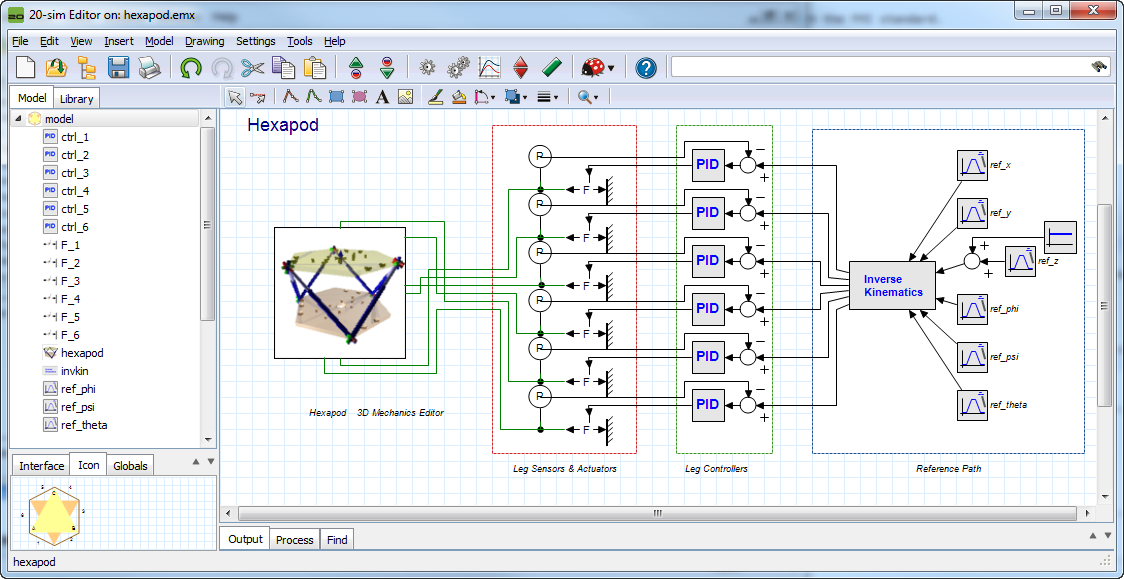
\includegraphics[width=\textwidth]{figures/20-sim_hexapod_model.png}}
	\caption{Example of a hexapod model in 20-sim.}
	\label{figure:20sim_hexapod_example}
\end{figure}
%
%
%
Figure \ref{figure:20sim_hexapod_example} shows {20-sim} with a model of a controlled hexapod.
%
The mechanism is generated with the 3D Mechanics Toolbox and connected with standard actuator and sensor models from the mechanics library.
%
The hexapod is controlled by PID controllers which are tuned in the frequency domain.
%
Everything that is required to build and simulate this model and generate the controller code for the real system is included inside the package.

The {20-sim} Getting Started manual \cite{20simGettingStarted16} contains examples and step-by-step tutorials that demonstrate the features of {20-sim}.
%
More information on {20-sim} can be found at \url{http://www.20sim.com} and in the user manual at \url{http://www.20sim.com/webhelp} \cite{20simReference16a}.
%
The integration of {20-sim} into the INTO-CPS tool-chain is realised via the FMI standard.
%
%
%
\subsection{OpenModelica}\label{app:OM}
OpenModelica \cite{Fritzson04} is an open-source Modelica-based modelling and simulation environment.
%
Modelica \cite{Fritzson&98} is an object-oriented, equation based language to conveniently model complex physical systems containing, e.g., mechanical, electrical, electronic, hydraulic, thermal, control, electric power or process-oriented subcomponents. The Modelica language (and OpenModelica) supports continuous, discrete and hybrid time simulations.
%
OpenModelica already compiles Modelica models into  FMU, C or C++ code for simulation.
%
Several integration solvers, both fixed and variable step size, are available in OpenModelica: euler, rungekutta, dassl (default), radau5, radau3, radau1.

OpenModelica can be interfaced to other tools in several ways as described in the OpenModelica user's manual \cite{OpenModelicaUG15}:
%
%
%
\begin{itemize}
%
\item via command line invocation of the omc compiler
%
\item via C API calls to the omc compiler dynamic library
%
\item via the CORBA interface
%
\item via OMPython interface \cite{Ganeson&12}
%
\end{itemize}
%
%
%
OpenModelica has its own scripting language, Modelica script (mos files), which can be used to perform actions via the compiler API, such as loading, compilation, simulation of models or plotting of results.
%
OpenModelica supports Windows, Linux and Mac Os X.

The integration of OpenModelica into the INTO-CPS tool chain is realised via compliance with the FMI standard, and is described in Deliverable D4.3b \cite{INTOCPSD4.3b}.
%
%
%
\subsection{RT-Tester}\label{app:RTT}
The RT-Tester \cite{VSI-rtt-man} is a test automation tool for automatic
test generation, test 
execution and real-time test evaluation. Key features include a strong
C/C++-based test script language, high performance multi-threading, and
hard real-time capability.
The tool has been successfully applied in avionics, rail automation, and
automotive test projects.
%
In the INTO-CPS tool chain, RT-Tester is responsible for model-based testing, as well as for model checking.
%
This section gives some background information on the tool from these two perspectives.
%
%
%
\subsubsection{Model-based Testing}
% RT-Tester Model Based Extension (RTT-MBT)
The RT-Tester Model Based Test Case and Test Data Generator (RTT-MBT) \cite{VSI-mbt-man} 
supports model-based testing (MBT), that is, automated generation of test cases, test
data, and test procedures from UML\allowbreak{}/SysML models. A number of common modelling
tools can be used as front-ends for this. 
%
The most important technical challenge in model-based test automation is the extraction of test cases from test models.
%
RTT-MBT combines an SMT solver with a technique akin to bounded model checking so as to extract finite paths through the test model according to some predefined criterion.
%
This criterion can, for instance, be MC/DC coverage, or it can be requirements coverage (if the requirements are specified as temporal logic formulae within the model).
%
A further aspect is that the environment can be modelled within the test model.
%
For example, the test model may contain a constraint such that a certain input to the system-under-test remains in a predefined range.
%
This aspect becomes important once test automation is lifted from single test models to multi-model cyber-physical systems.
%
The derived test procedures use the RT-Tester Core as a back-end, allowing the
system under test to be provided on real hardware, software only, or even
just simulation to aid test model development.

Further, RTT-MBT includes requirement tracing from test models down to test executions
and allows for powerful status reporting in large scale testing projects.
%
%
%
\subsubsection{Model Checking of Timed State Charts}
\label{appendix:rtt-model-checking}
RTT-MBT applies model checking to behavioural models that are specified as timed state charts in UML and SysML, respectively.
%
From these models, a transition relation is extracted and represented as an SMT formula in bit-vector theory~\cite{Kroening&08}, which is then checked against LTL formulae~\cite{Pnueli77} using the algorithm of Biere \emph{et al.\@}~\cite{Biere&06}.
%
The standard setting of RTT-MBT is to apply model checking to a single test model, which consists of the system specification and an environment.
%
%
%
\begin{itemize}
%
\item A component called \emph{TestModel} that is annotated with stereotype \emph{TE}.
%
\item A component called \emph{SystemUnderTest} that is annotated with stereotype \emph{SUT}.
%
\end{itemize}
%
%
%
RTT-MBT uses the stereotypes to infer the role of each component.
%
The interaction between these two parts is implemented via input and output interfaces that specify the accessibility of variables using UML stereotypes.
%
%
%
\begin{itemize}
%
\item A variable that is annotated with stereotype \emph{SUT2TE} is written by the system model and readable by the environment.
%
\item A variable that is annotated with stereotype \emph{TE2SUT} is written by the environment and read by the system model as an input.
%
\end{itemize}
%
%
%
A simple example is depicted in \autoref{figure:vsi-simple}, which shows a simple composite structure diagram in Modelio for a turn indication system.
%
The purpose of the system is to control the lamps of a turn indication system in a car.
%
Further details are given in~\cite{rttmbtmanual}.
%
The test model consists of the two aforementioned components and two interfaces:
%
%
%
\begin{itemize}
%
\item {\bf Interface1} is annotated with stereotype \emph{TE2SUT} and contains three variables {\tt voltage}, {\tt TurnIndLvr} and {\tt EmerSwitch}. These variables are controlled by the environment and fed to the system under test as inputs.
%
\item {\bf Interface2} is annotated with stereotype \emph{SUT2TE} and contains two variables {\tt LampsLeft} and {\tt LampsRight}. These variables are controlled by the system under test and can be read by the environment.
%
\end{itemize}
%
%
%
Observe that the two variables {\tt LampsLeft} and {\tt LampsRight} have type {\tt int}, but should only hold values {\tt 0} or {\tt 1} to indicate states \emph{on} or \emph{off}.
%
A straightforward system property that could be verified would thus be that {\tt LampsLeft} and {\tt LampsRight} indeed are only assigned {\tt 0} or {\tt 1}, which could be expressed by the following LTL specification:
%
%
%
\[
\mathbf{G} (0 \leq {\tt LampsLeft} \leq 1 \wedge 0 \leq {\tt LampsRight} \leq 1)
\]
%
%
%
A thorough introduction with more details is given in the RTT-MBT user manual~\cite{rttmbtmanual}.
%
%
%
\begin{figure}
\centerline{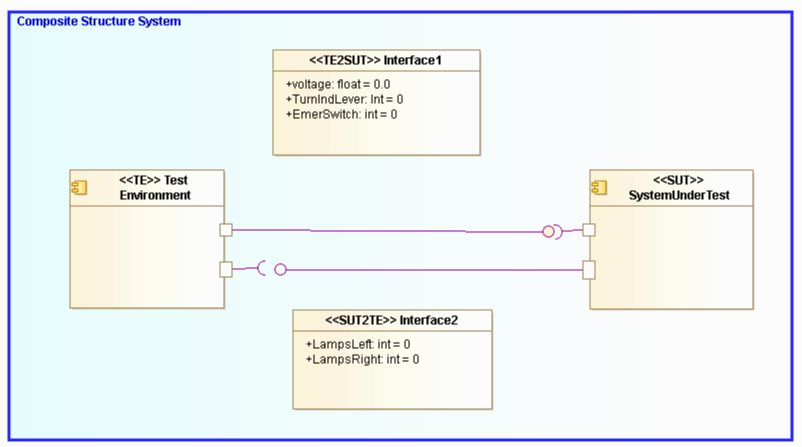
\includegraphics[width=\textwidth]{figures/VSI-modelio_turn_indication_small_toplevel_composite.png}}
\caption{Simple model that highlights interfaces between the environment and
  the system-under-test.}
\label{figure:vsi-simple}
\end{figure}

\subsection{4DIAC}

\fbox{Jose Cabral}

\subsection{AutoFOCUS-3}

\fbox{Jose Cabral}

%
%
%
\end{document}
